\chapter{Models of Temperature Distributions in Pebble Beds}\label{sec:dem-studies}

This chapter demonstrates the usefulness of the numerical tools introduced in \cref{ch:modeling-development} in probing inter-particle contact information, pebble bed heat transfer, and bed morphology changes altering thermophysical properties. The DEM, CFD-DEM, and DEM-LBM tools are put to work examining representative volumes of pebble beds of ceramic breeders from fusion reactors. In almost all cases, the pebble bed volumes accommodate approximately \num{10000} pebbles. Typically, the bed is confined in one direction by two primitive, rigid walls that also are constant temperature boundaries to act as heat sinks. I also employ periodic boundary conditions to represent an infinite length in the given direction. The third direction is often in the gravity direction for which we have an adiabatic, primitve, and rigid roof and ceiling.

The first study considers the heat transfer in a pebble bed purely through contact conduction of grains in the ensemble. In this pebble bed, I employ DEM tools to apply a nuclear heating source and allow the bed to reach a thermal steady-state with the cooling walls. In such a way, an effective thermal conductivity of the bed is determinable. I then induce a fictitious pebble damaging method to the bed and check the changes to effective thermal conductivity. The DEM tools are used to then interrogate many micromechanical interactions in the pebble bed which we use to deduce the source of changes to the effective thermal conductivity.

In the second study, the same pebble bed is analyzed but this time the helium purge gas is included via the coupled CFD-DEM tools. I again induce some fictitious damage to the pebble bed and monitor changes to the thermophysical properties and their relationship to the cases when the helium purge gas was neglected. The study reveals important features of the helium influence on heat transfer in the bed.

In the third study, I take snapshots of two beds (a standard bed and a damaged one) and load them into LBM models. With lattice-Boltzmann it is possible to analyze the tortuous path of helium moving through the pebble bed and discover interesting features of the purge gas thermal interaction that was masked by the simplifications of the volume-average approach of CFD-DEM.



%%%%%%%%%%%%%%%%%%%%%%%%%%%%%%%%%%%%%%%%%%%%%%%%%%%%%%%%%%%%%%%%%%%%%%%%%%%%%%%%%%%%%%%%%%%%%%
\section{DEM Study on Effective Conductivity of Pebble Peds with Pebble Damage}\label{sec:dem-studies-effective-conductivity}
% The discrete element method (DEM) is used by many ceramic breeder researchers to model the interaction of individual pebbles in an ensemble in an effort to obtain a more detailed understanding of pebble beds than is possible with experimental measurements of effective properties. For example see Refs.~\cite{An20071393, Lu2000, Zhao2010, Gan:2010uq, Annabattula2012a, VanLew2014}.

% The discrete element method has been used for studies in a variety of fields for studying inter-particle forces and the homogeneously distributed force networks that arise in packed beds.\cite{Makse2000} 

The discrete element method has been used by researchers in the fusion community to attempt modeling crushing initiation and propagation\cite{Annabattula2012a, Zhao2012, Zhao2013}. They observed that a relatively few number of high-force networks, distributed throughout the bed supported the external mechanical loads. The even distribution of the force networks was used to defend the development of a probability-based predictor for crushing by Zhao\etal.\cite{Zhao2013} The basic premise is that probability distributions of strength curves for pebble crushing have been observed (see, for example crush loads of Ref.~\cite{Tsuchiya1998}). Then in DEM models, a probability distribution of inter-particle forces are also observed. Overlaying the two probabilities resulted in seemingly random locations of pebbles satisfying the damage criteria -- not strictly along the high-force chains running through packed beds.

To separate studies of crushing initiation from its downstream effects on mechanical and thermal properties, I make use of results of Zhao\etal~to create fictitiously damaged beds without consideration of the initiation of the damage. Zhao\etal~found that, with their predictive tool, pebbles are crushed in random locations. If this is the case, I may de-couple the task of predicting pebble damage (\textit{i.e.} finding the mechanical or thermal load that causes a pebble to fail) from the task of modeling the ramifications of pebble crushing. I am free to randomly assign pebble damage to mimic the random locations from predictions. This is how I will model pebble damage in this first model.

As far as modeling the fragmentation, I begin with an extreme assumption of pulverization of the particle -- a not entirely unrealistic assumption. Experiments on crushing single, brittle pebbles reveal that there are a number of failure modes.\cite{Wu2004} At one extreme, the pebble may simply crack and continue to hold a load for some time. At the other extreme, a pebble may crush practically into a dust. The damage method used in this study is an extension of that latter extreme. When a pebble in our simulation has been flagged for damage, it is completely removed from the ensemble. The remaining pebbles are allowed to rearrange to compensate for the lack of equilibrium on their contact forces due to the missing pebbles. In later models I will use the fragmentation approach as outlined in \cref{sec:failure-study}.


\subsection{Model Setup \& Methodology}\label{sec:dem-setup}
I analyze a three-dimensional pebble bed consisting of mono-dispersed particles of diameter $d_p$. The particles are constrained by rigid $y$-$z$-planes at locations of $\frac{x}{d_p} = \pm 10$ (the walls of the container). There are periodic boundary conditions in the $y$-direction located at $\frac{y}{d_p} = \pm 7.5$. Gravity acts in the negative $z$-direction and the particles are resting on a rigid $x$-$y$-plane at $z=0$ (the floor of the container) and held from the top by an $x$-$y$-plane at $\frac{z}{d_p} = 30$ (the roof of the container). It is packed to $\phi = 64\%$ and, given the volume, have 11000 particles. The volume was chosen to represent the long, tall, narrow channels seen in many solid breeder module designs\cite{ Cho2008, Poitevin2010, Enoeda2003}.

For this study, the material properties were chosen to represent lithium metatinatate pebbles. All the properties come from Ref.~\cite{Gierszewski1998}. They are summarized in Table~\ref{tab:mat-props}

\begin {table}[tp] %
\caption{Maximum load and nominal tension.}
\label {tab:mat-props} \centering %
\begin {tabular}{ cccccc }
\toprule %
E           &     $\nu$     &    k          &    C          &   $\alpha$                \\
(\si{\giga\pascal})     &               & (\si{\watt\per\meter\per\kelvin})         &  (\si{\joule\per\kilogram\per\kelvin})    &   (\si{\per\kelvin})                   \\\toprule
\num{126}           &      \num{0.24}     &  \num{2.5}          &  \num{1156}           &   \num{15e-6}     \\\bottomrule
\end{tabular}
\end{table}

% In the first attempt at packing pebbles into the system, we begin with a common starting point of a filled, lightly packed volume of 10~550 pebbles. We simulate pouring the pebbles into the volume by initializing them into the system from a height of $\frac{z}{d_p} \approx 50$ and allow them to fall under the influence of gravity (see \Cref{fig:fill01}). We pack the pebbles into a higher packing fraction by means of oscillating the walls as if the pebble bed were sitting on a vibrating plate. This was to imitate the vibration packing technique done in our experimental lab when testing pebble beds in the uniaxial compression test stand. The vibration scheme was able to slowly densify the packed bed but, owing to the very small time step of the simulation, the simulation times were impractically large to approach a packing fraction greater than $\phi = 60\%$. 

\begin{figure}[!ht]
    \centering
    \begin{subfigure}[b]{0.25\textwidth}
        \centering
        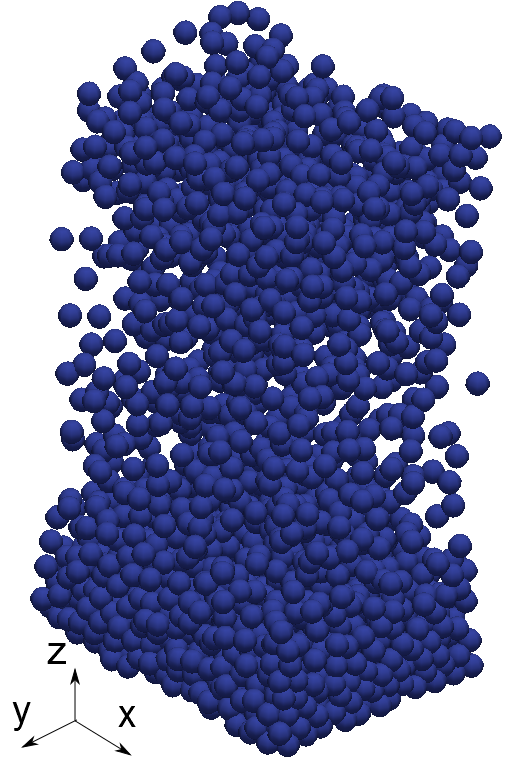
\includegraphics[width=\textwidth]{figures/fill01.png}
    \end{subfigure}
    \begin{subfigure}[b]{0.25\textwidth}
        \centering
        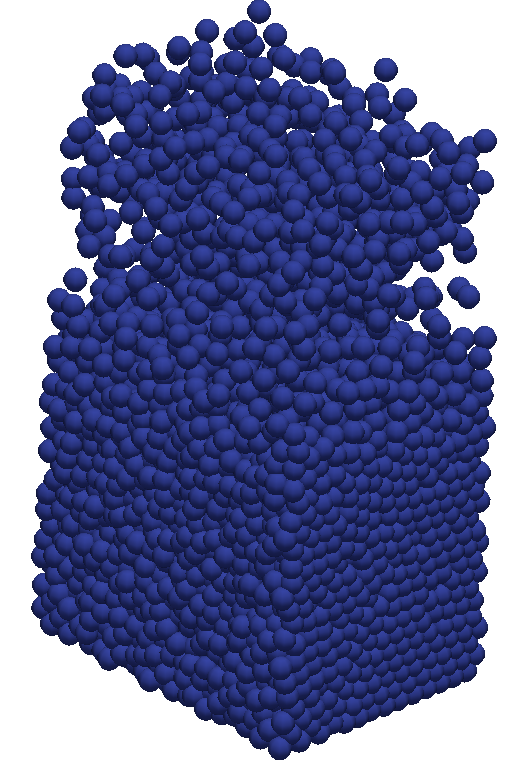
\includegraphics[width=\textwidth]{figures/fill02.png}
    \end{subfigure}
    \begin{subfigure}[b]{0.25\textwidth}
        \centering
        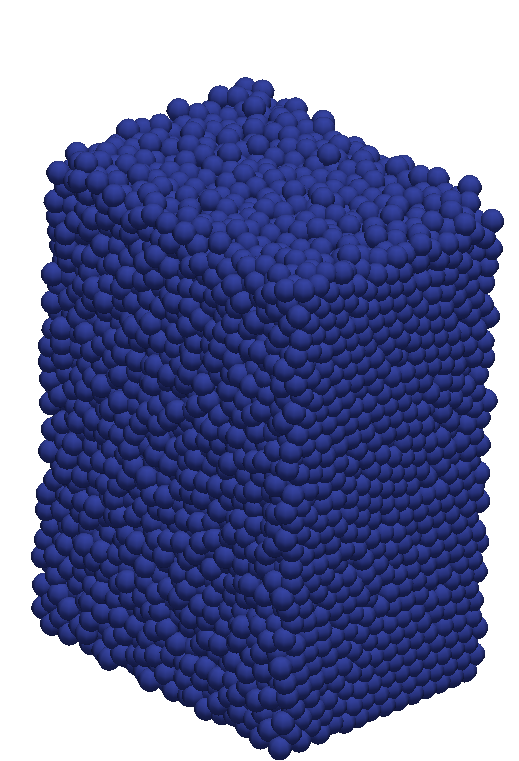
\includegraphics[width=\textwidth]{figures/fill03.png}
    \end{subfigure}
    \caption{Demonstrating the pouring process of $N = 10550$ pebbles into the control volume with at an early time (left), when it is nearly filled (middle) and after the pebbles have settled to negligible kinetic energy (right).}
\label{fig:fill01}
\end{figure}

The first attempt to pack the bed followed from the `recipes' we had used in physical experiments in the lab. That is, the pebbles were numerically poured into the volume from above and allowed to settle under their own weight (see \Cref{fig:fill01}), then the volume was vibrated while a roof was lowered to compact the system to $\phi = 0.64$, the desired packing fraction. This technique was ultimately abandoned in place of a less realistic but more computationally efficient technique which resulted in comparably packed beds.

In the preferred method, $N$ particles are inserted into the volume such that we have precisely the packing fraction we desire. In this case, $\phi = 0.64$ so $N$ = \num{11000}. The pebbles are placed at random into the volume, allowing artificial overlap -- often by a great deal ($\delta$ on the order of $R_p$). The overlap they experience would normally cause such an enormous force (integrating into an enormous velocity) that the pebbles would all explode out of the bed at the first step in time integration. The catastrophic explosion is avoided with a relaxation scheme wherein the displacement of any pebble per time step, as integrated from force, is truncated. The truncated displacement continues slowly and allows the pebbles to slowly move away from each other and into a static equilibrium as the artificial overlap is reduced. Once the pebble bed comes to rest, I remove the relaxation (limiting displacement command) and the standard integration of contact forces with the velocity-Verlet algorithm is re-initiated. The pack-relax scheme allowed for obtaining desirable, highly repeatable packing fractions for all pebble beds. Once the pebble bed was packed into an initial condition, the simulation state was saved and used as a starting point for the numerous `crushed' cases to be described later. I differentiate the failed beds by their percentage of failed pebbles: $\eta = $ number of failed pebbles per original ensemble size.

%In this first study, we model pebble crushing without considering why the particular pebble should be cracking. In the model we randomly select pebbles from the ensemble, regardless of forces acting upon the pebble, and delete them entirely from the system. When a pebble is removed, the neighboring pebbles react due to the imbalance of forces, and the bed settles into a new configuration. 

To simulate the conditions of a solid breeder in a fusion reactor, where the heat is removed from the pebble bed via contact to the containing structure, I assign a constant temperature of $T_\text{c}$ to the vertical walls. Nuclear heating of the pebbles is simulated through a constant source term on each pebble. A representative heating rate of $Q_s = q_p'''V_p$, where  $q_p'''= 8$ MW/m$^3$. The heating cycle runs until a thermal steady state is reached. Based on a measurement of the total thermal energy of the bed, $E_T =\sum_i^N m_iC_i T_i$, steady-state is determined as $\dt{E_T} = 0$ within a specified tolerance. Once at steady state, I analyze thermal and mechanical characteristics of the pebble bed: effective thermal conductivity, average coordination number, temperature profiles in the bed, and inter-particle contact forces. 

Based on the boundary conditions of the system, the heat transfer becomes symmetric and one-dimensional in the $x$-direction from $x=0$ to the walls at $\frac{x}{d_p} = \pm 10$. As we will see, the pebble bed has very little variation of forces and temperatures in the $y$-direction due to the periodic boundary condition at the edges of the domain. Gravity effects are minor in the overall heat transfer and induce only a slight $z$-dependency to the results. I take advantage of the pebble bed temperature profile's resemblance to a one-dimensional heat transfer problem to calculate an effective conductivity from an analytic, one-dimensional test case analogy.
%~~~~~~~~~~~~~~~~~~~~~~~~~~~~~~~~~~~~~~~~~~~~~~~~~~~~~~~~~~~~~~~~~~~~~~





%~~~~~~~~~~~~~~~~~~~~~~~~~~~~~~~~~~~~~~~~~~~~~~~~~~~~~~~~~~~~~~~~~~~~~~
\subsection{Effective Thermal Conductivity from Analytic Analogy}\label{sec:keff-analogy}
Assuming a one-dimensional pebble bed, to find an effective conductivity, we step back into a continuum mechanics formulation where the pebble bed can be represented as a slab of solid material. We can analytically solve for the temperature equation in a slab with heat generation, symmetry about the centerline, and a constant boundary temperature condition.

At steady-state, the temperature of a material with constant temperature boundary conditions ($T(L) = T_s$), constant thermal conductivity ($\keff$), and nuclear heating ($q'''$) obeys the following equation

\begin{equation}\label{eq:continuum-heateqn}
    0 = \frac{\mathrm{d}^2T}{\mathrm{d}x^2} + \frac{q'''}{\keff}
\end{equation}

In nondimensional form, the temperature is
\begin{equation}
    \theta = \frac{T(x) - T_s}{T_0 - T_s}
\end{equation}
where $T_0$ is the temperature at the centerline of this slab (a value found momentarily). The length is nondimensionalized as
\begin{equation}
    x^* = \frac{x}{L}
\end{equation}

Thus \Cref{eq:continuum-heateqn} in nondimensional form is,
\begin{equation}\label{eq:continuum-heateqn-nondim}
    0 = \frac{\mathrm{d}^2\theta}{\mathrm{d}x^{*2}} + G
\end{equation}
where
\begin{equation}
    G = \frac{q'''L^2}{\keff(T_0 - T_s)}
\end{equation}

In the nondimensionalized form, the solution is revealed to be purely geometric,
\begin{equation}\label{eq:continuum-temperature-nondim}
    \theta = 1-x^{*2}
\end{equation}
as $T_0  - T_s = \frac{q'''L^2}{2\keff}$. I will use the nondimensional temperature solution of \Cref{eq:continuum-temperature-nondim} to prove the one-dimensional assumption of heat transfer is justified for the pebble beds.

Noting that in this continuum mechanics formulation, we are assuming that the nuclear source, $q'''$ term is applied evenly over the entire volume. In our DEM formulation, our source term applies to a single pebble. To find the effective thermal conductivity of the `slab' of pebble bed, we must reconcile this discrepency. This is accomplished with the exchange of
\begin{equation}\label{eq:q-source-translation}
    q''' = \frac{Q_\text{tot}}{V_\text{tot}} = \frac{Q_sN}{H\cdot L\cdot W\cdot d_p^2}
\end{equation}
where the pebble bed volume is given by the height, $H$, width, $W$, and length, $L$, and $Q_s$ is the source term on each pebble in the DEM ensemble. 

From the solution of \Cref{eq:continuum-heateqn-nondim}, we find the effective conductivity to be
\begin{equation}
    \keff = \frac{q''' L^2}{2(T_0-T_s)}
\end{equation}
and when we replace the heat generation term with \Cref{eq:q-source-translation}, and use the bed dimensions as given in \cref{sec:dem-setup}, this is written as
\begin{equation}\label{eq:dem-effecitve-conductivity-formula}
    \keff = \frac{Q_sN}{180(T_0-T_s)d_p}
\end{equation}

I use this formulation of \Cref{eq:dem-effecitve-conductivity-formula} to analyze and compare the pebble beds of this study.
% \begin{figure}[htbp]
%   \centering
%   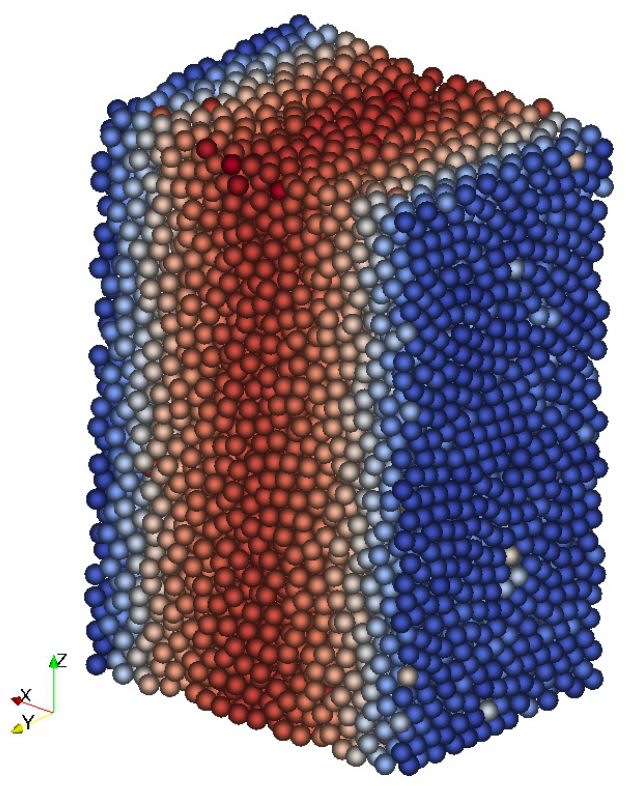
\includegraphics[trim=1cm 8cm 3cm 4cm, width=0.5\textwidth]{figures/pebbleBedTemperature}
%   \caption{Temperature distribution of pebbles in the $10\%$ failed bed. At the end of steady-state heating, a one-dimensional profile is evident in all pebble beds studied here. The pebbles are receiving nuclear heating. Cooling proceeds through the pebbles in contact with the walls in the $x$-direction.}
% \label{fig:pebbleBedTemperature}
% \end{figure}



\subsection{Results}
The aim of this study was both to discover the impact of pebble failure on thermo-mechanical properties as well as determine the impact as a function of the number of failed pebbles. To satisfy the latter, I created beds with $\eta = 1\%$, $3\%$, $5\%$, $10\%$, and $15\%$ of pebbles failed. 

I plot \Cref{eq:continuum-temperature-nondim} against the nondimensionalized temperature profiles coming from the steady-state DEM simulation in \Cref{fig:temp-scatters}. We see that all the models had a nearly perfect match to a one-dimensional prediction, validating the calculation of effective thermal conductivity in this study. Furthmore, the profiles adhering to the one-dimensional curve also allows us to find the effective conductivity of each bed from applying \Cref{eq:dem-effecitve-conductivity-formula}, which was derived from the one-dimensional assumption.

In a well-packed bed, most pebbles have a coordination number $Z > 6$. But even in a well-packed bed, there exist some `rattlers' -- pebbles that have only 1 or 2 contact points (aside from touching the floor or wall). These rattlers, without strong contact to neighbors, heat up arbitrarily high in the system. In a pebble bed that's resettling due to damage, increased numbers of rattlers appear in the bed. The isolated rattlers are apparent in the scatter plots of \Cref{fig:temp-scatters}. The temperatures of most pebbles are tightly grouped around the parabolic average. Though many data points are seen dotted all around the temperature scale. The phenomena of hot rattlers is only possible when we use DEM without consideration of the helium purge gas. If these hot rattlers persist even in the presence of helium, it could lead to an unfavorable performance of the ceramic solid breeder -- the hot rattlers would sinter and prevent the outgassing of tritium among other issues. The observation of these isolated pebbles is another motivator for the coupling of DEM to thermo-fluid models. Because the 10\% and 15\% cases have such high temperatures, we show only the 0-5\% crushed together in \Cref{fig:temp-scatters-zoomed}

\begin{figure}[htbp]
    \centering
    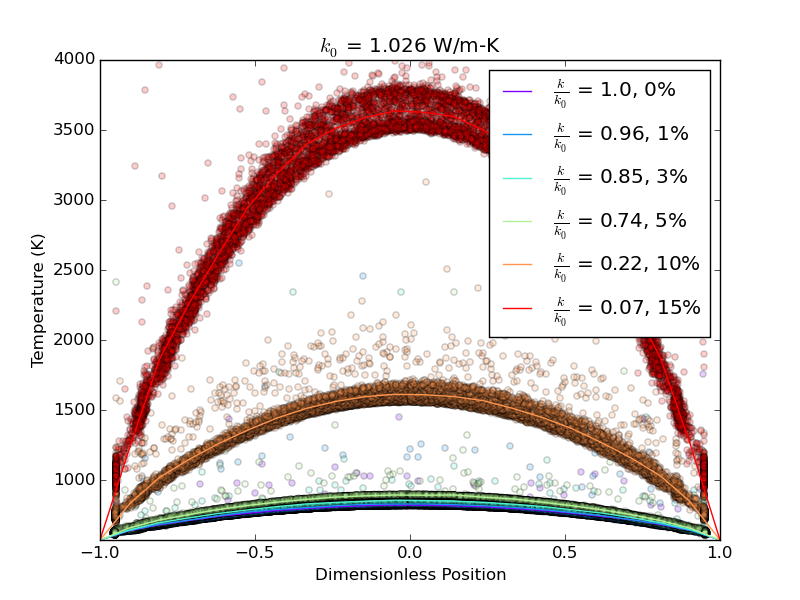
\includegraphics[width=\singleimagewidth]{figures/dem-evap-0-15-scatter-keff.png}
    \caption{The nondimensional temperature profiles for each test case follow the theoretical shape of a one-dimensional, constant $k$, continuum solution.}
\label{fig:temp-scatters}
\end{figure}

\begin{figure}[htbp]
    \centering
    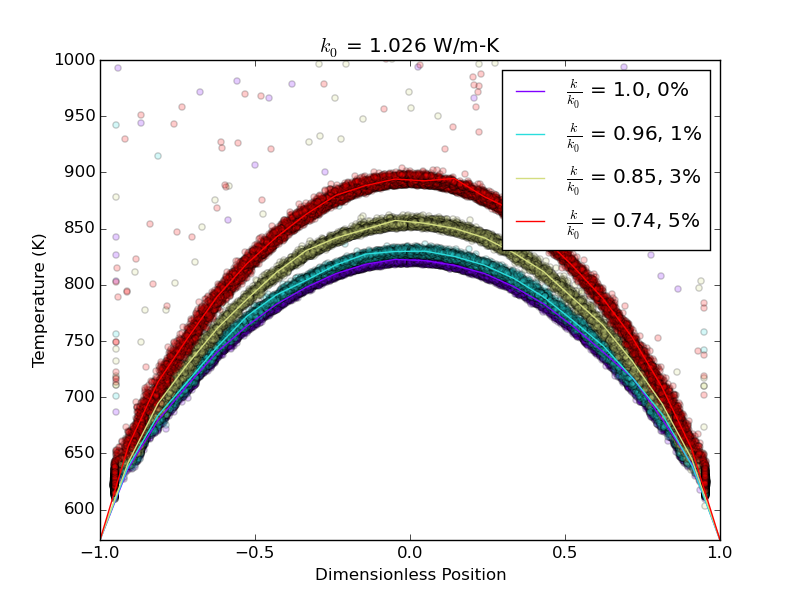
\includegraphics[width=\singleimagewidth]{figures/dem-evap-0-5-scatter-keff.png}
    \caption{The nondimensional temperature profiles for the test cases up to 5\% crushed pebbles.}
\label{fig:temp-scatters-zoomed}
\end{figure}


In order to calculate an effective conductivity of the pebble bed, I find an average temperature profile through the bed to compare with \Cref{eq:continuum-temperature-nondim} and thus employ \Cref{eq:dem-effecitve-conductivity-formula}. Average values of the bed, along the $x$ direction, are generated via averaging temperatures in bins. I create bins that are volumes slices of width $\Delta x$ that extend through the limits of the $y$- and $z$-directions. I then find the $n$ pebbles residing in the slices and take the mean value of their temperatures. The average, given by \Cref{eq:binned-T}, is also shown as the solid lines in \Cref{fig:temp-scatters}. The binned average temperature is 
\begin{equation}\label{eq:binned-T}
    \langle T\rangle = \frac{1}{n}\sum_{i}^n T_i    
\end{equation}
Using the volume slices, I also find the average coordination number, 
\begin{equation}\label{eq:binned-z}
    \langle Z \rangle = \frac{1}{n}\sum_{i}^n Z_i
\end{equation}
and average contact force, 
\begin{equation}\label{eq:binned-f}
    \langle F^{1/3} \rangle = \frac{1}{n}\sum_{i}^n F_{n,ij}^{1/3}
\end{equation}


In \Cref{eq:thermoFirstLaw} of \cref{sec:dem-heat-transfer}, we see that at steady-state, the energy input by nuclear heating must be balanced by the transport of heat out of a pebble into its neighbors. Inter-particle heat transfer is dictated by the number of neighboring contacts, temperature difference between pebbles, and the thermal conductance, $H_{c}$, through the contact area. The thermal conductance is itself a function purely of material properties  (which are essentially constant here) and the force at the contact, going as $H_{c} \propto F_{n,ij}^{1/3}$. Thus, I write the net heat out of a pebble at steady state as a function of the three variables,

\begin{equation}
    Q_\text{net} =f( Z, F_n^{1/3}, \Delta T)
\end{equation}

The coordination number and contact forces are features of the packing structure in the packed bed that we can analyze to discover what happens to the heat flux between pebbles when the bed experiences crushed particles. Conversely, the $\Delta T$ between two pebbles is the \textit{effect} of the thermal transport (\textit{i.e.} leading to higher bed temperatures such as those of \Cref{fig:temp-scatters}). We will first analyze the changes to the coordination numbers of pebbles in the ensemble as pebbles crush.


\begin{figure}[!ht]
    \centering
    \begin{subfigure}[b]{\doubleimagewidth}
        \centering
        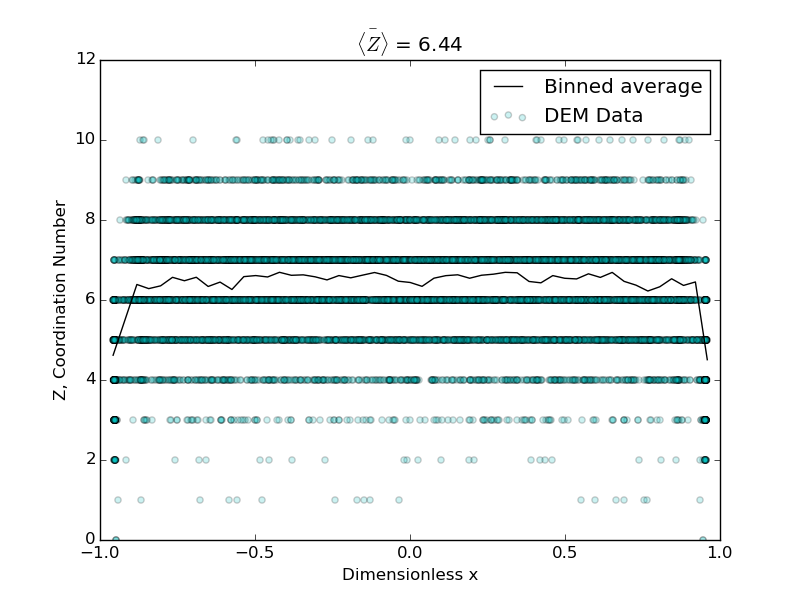
\includegraphics[width=\textwidth]{figures/heating_dte-02/dem-evap-0-scatter-coord.png}
        \caption{Baseline pebble bed (0\% crushed)}
    \end{subfigure}
    \begin{subfigure}[b]{\doubleimagewidth}
        \centering
        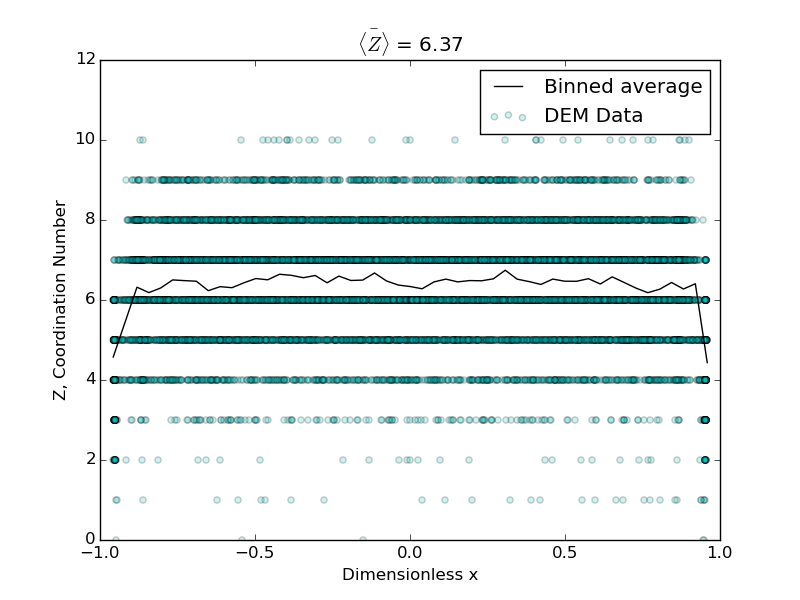
\includegraphics[width=\textwidth]{figures/heating_dte-02/dem-evap-1-scatter-coord.png}
        \caption{1\% crushed}
    \end{subfigure}
    
    \begin{subfigure}[b]{\doubleimagewidth}
        \centering
        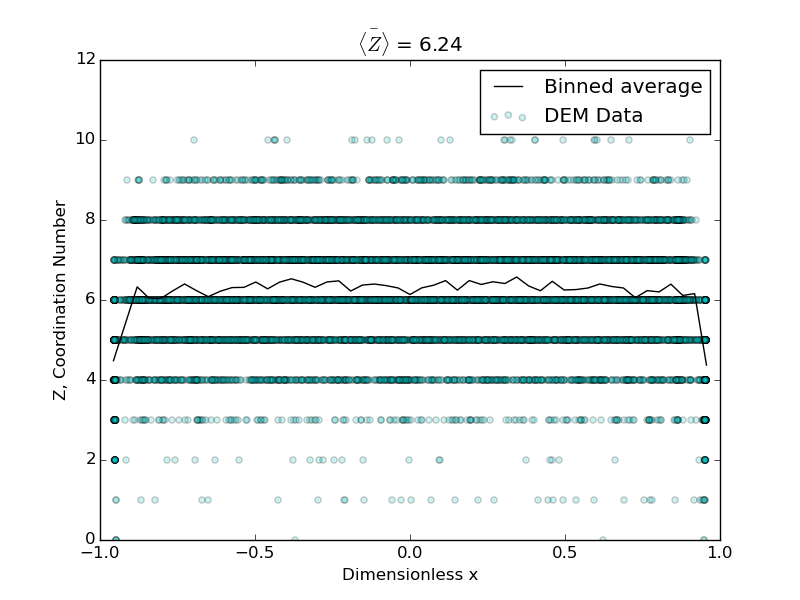
\includegraphics[width=\textwidth]{figures/heating_dte-02/dem-evap-2-scatter-coord.png}
        \caption{3\% crushed}
    \end{subfigure}
    \begin{subfigure}[b]{\doubleimagewidth}
        \centering
        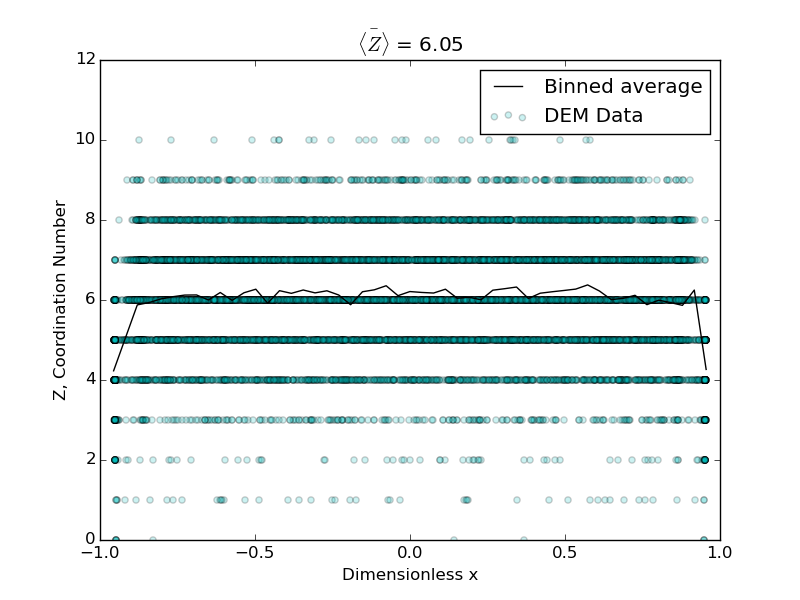
\includegraphics[width=\textwidth]{figures/heating_dte-02/dem-evap-3-scatter-coord.png}
        \caption{5\% crushed}
    \end{subfigure}

    \begin{subfigure}[b]{\doubleimagewidth}
        \centering
        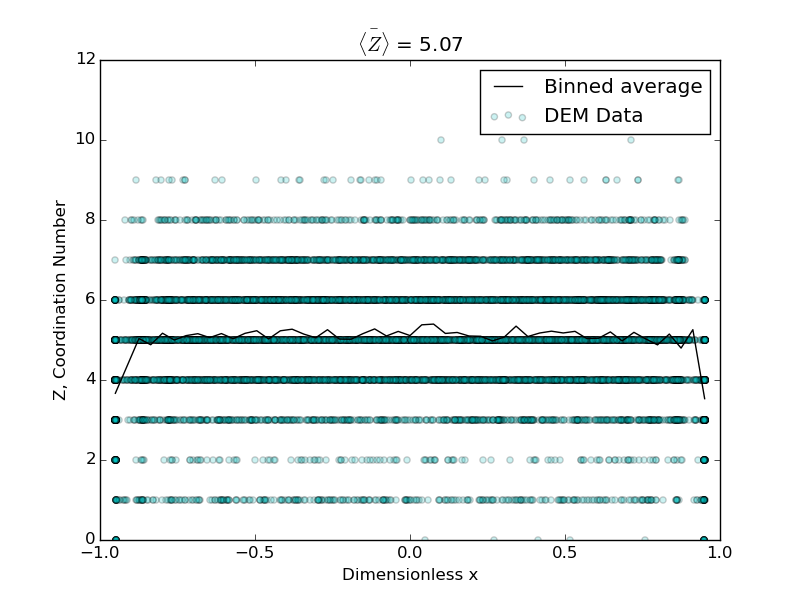
\includegraphics[width=\textwidth]{figures/heating_dte-02/dem-evap-4-scatter-coord.png}
        \caption{10\% crushed}
    \end{subfigure}
    \begin{subfigure}[b]{\doubleimagewidth}
        \centering
        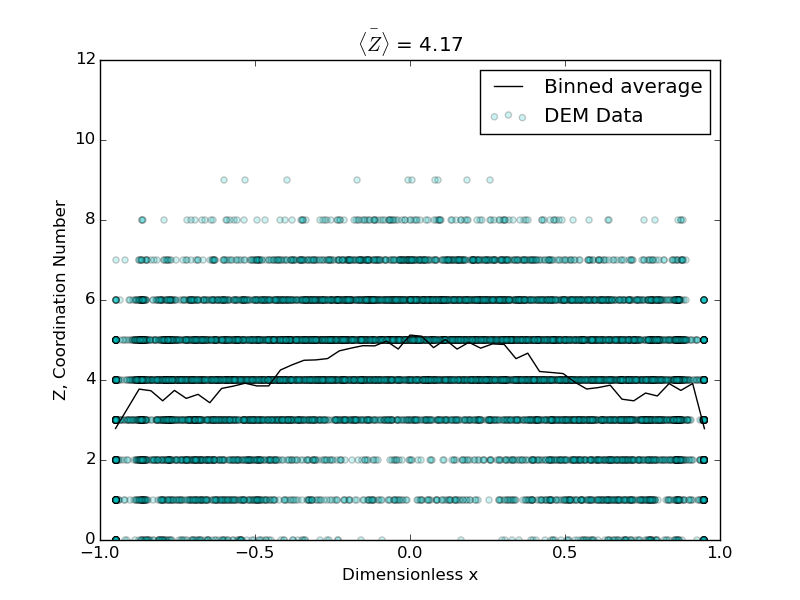
\includegraphics[width=\textwidth]{figures/heating_dte-02/dem-evap-5-scatter-coord.png}
        \caption{15\% crushed}\label{fig:coord-scatter-15percent}
    \end{subfigure}
    \caption{The average coordination number decreases slowly as the number of broken pebbles in the ensemble increases.}
\label{fig:coord-scatter}
\end{figure}

In \Cref{fig:coord-scatter} we plot the data for all pebbles in the ensemble as well as the binned average (\Cref{eq:binned-z}). Clearly, there are fewer average contacts per pebble in the ensemble after failure; At 15\% crushed the coordination number drops by roughly 30\%. The normal contact forces between pebbles are plotted in \Cref{fig:contact-forces-scatter}. A dramatic reduction in the normal forces is seen after many of their neighbors are crushed and are removed from the system. From the baseline down to the 15\% failed case, the contact forces are reduced by about a factor of 10 - similar to the reduction in effective conductivity.


\begin{figure}[!ht]
    \centering
    \begin{subfigure}[b]{0.4\textwidth}
        \centering
        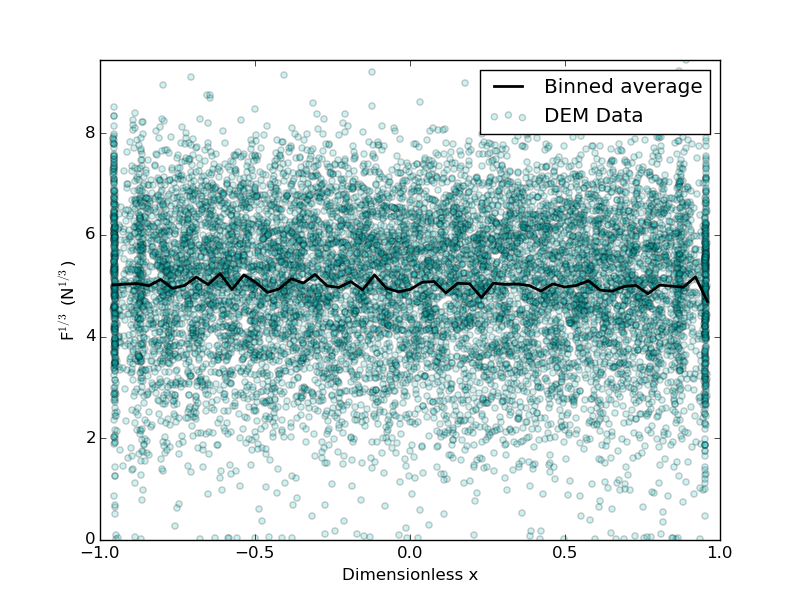
\includegraphics[width=\textwidth]{figures/heating_dte-02/0/dump/force-profile.png}
        \caption{Baseline pebble bed (0\% crushed)}
    \end{subfigure}
    \begin{subfigure}[b]{0.4\textwidth}
        \centering
        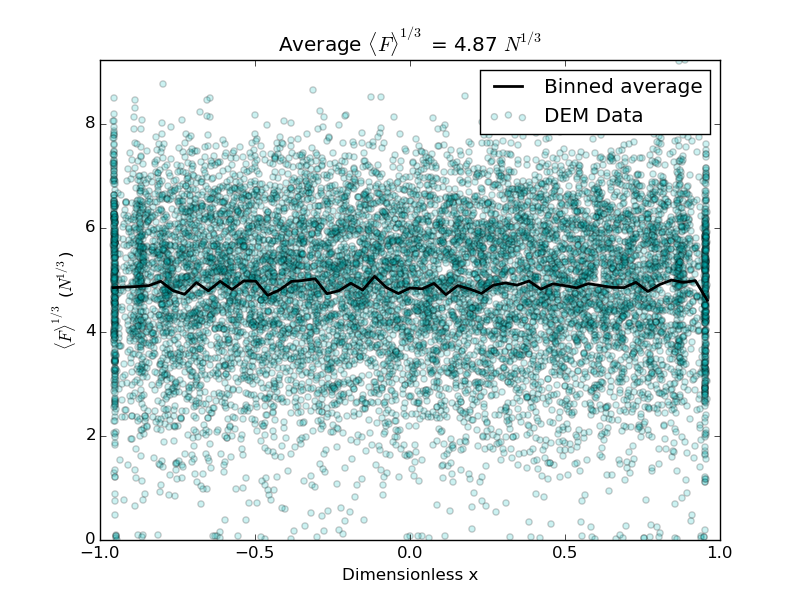
\includegraphics[width=\textwidth]{figures/heating_dte-02/1/dump/force-profile.png}
        \caption{1\% crushed}
    \end{subfigure}
    
    \begin{subfigure}[b]{0.4\textwidth}
        \centering
        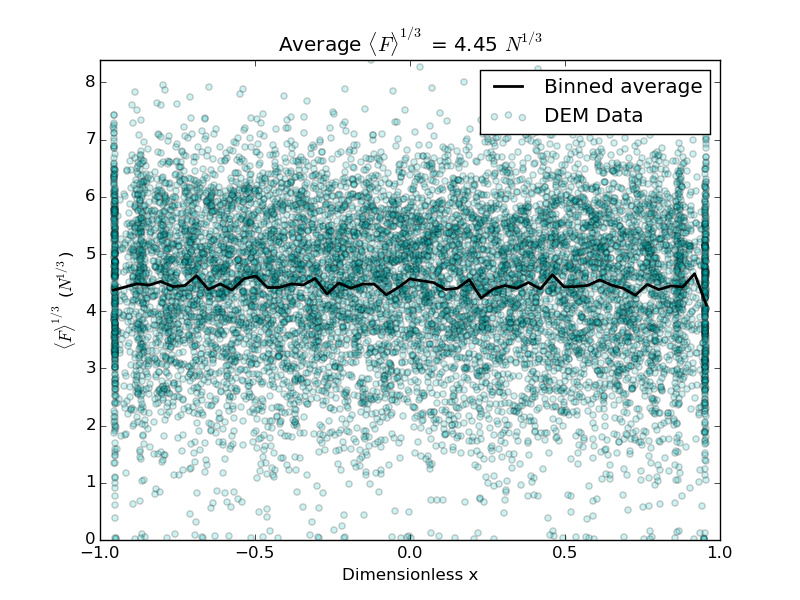
\includegraphics[width=\textwidth]{figures/heating_dte-02/3/dump/force-profile.png}
        \caption{3\% crushed}
    \end{subfigure}
    \begin{subfigure}[b]{0.4\textwidth}
        \centering
        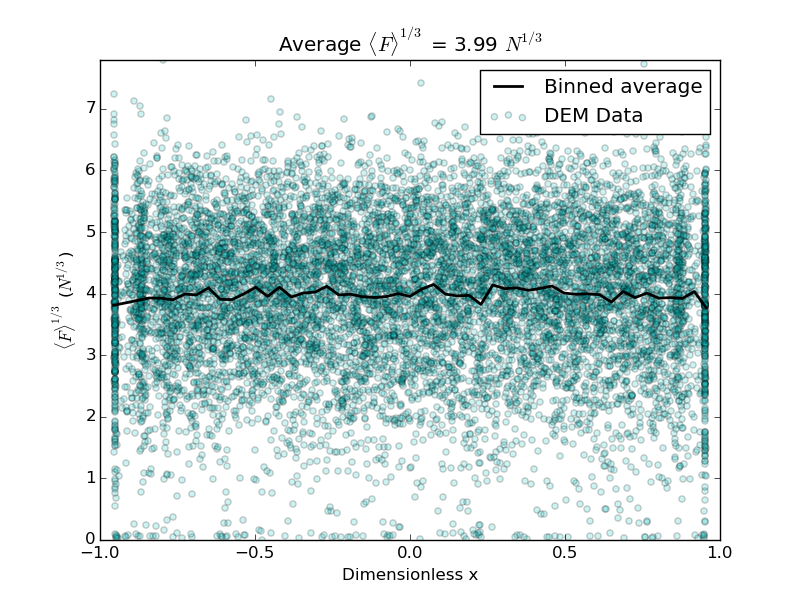
\includegraphics[width=\textwidth]{figures/heating_dte-02/5/dump/force-profile.png}
        \caption{5\% crushed}
    \end{subfigure}

    \begin{subfigure}[b]{0.4\textwidth}
        \centering
        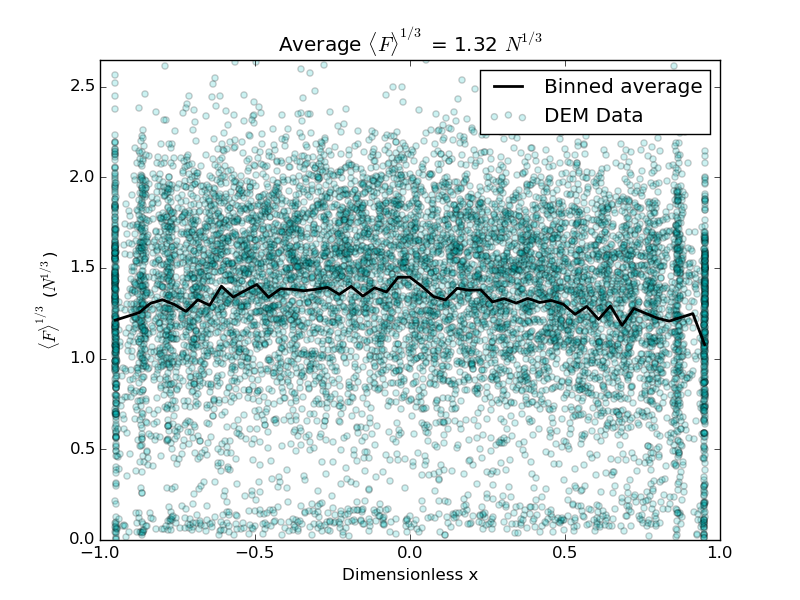
\includegraphics[width=\textwidth]{figures/heating_dte-02/10/dump/force-profile.png}
        \caption{10\% crushed}
    \end{subfigure}
    \begin{subfigure}[b]{0.4\textwidth}
        \centering
        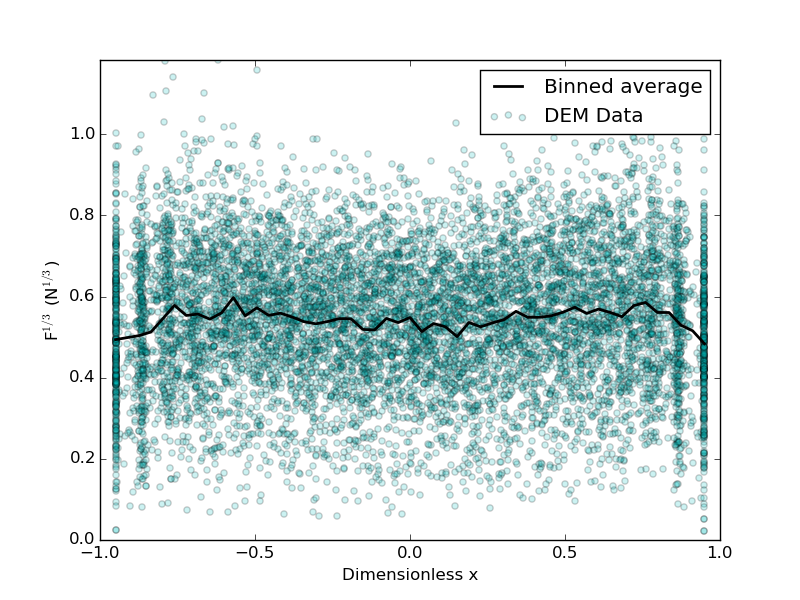
\includegraphics[width=\textwidth]{figures/heating_dte-02/15/dump/force-profile.png}
        \caption{15\% crushed}\label{fig:contact-forces-scatter-15percent}
    \end{subfigure}
    \caption{As pebble beds experience massive amounts of crushed pebbles (>5\%), the contact forces in the ensemble (after heating to steady-state) show dramatic reductions in value. Note the change of scale on the figures from the baseline case to the 15\% crushed case.}
\label{fig:contact-forces-scatter}
\end{figure}



The effective thermal conductivity was found for all of the pebble beds, via \Cref{eq:dem-effecitve-conductivity-formula}, then normalized against the conductivity of the baseline ensemble ($k^* = k/k_\text{0}$). The average coordination number of the beds and average normal contact forces were also found. Another way of describing a pebble bed is with the packing fraction, $\phi$. In \Cref{fig:packing-fraction}, I collect all these values (and normalize them against the baseline case) to provide a direct comparison to their changes as a function of crushed pebbles. When $15\%$ of the pebbles are crushed in a pebble bed, the effective conductivity has fallen all the way to only $k^*=0.07$. This large reduction is especially important in light of the already poor thermal management of virgin pebble beds that, even in helium environments, have been experimentally measured at only approximately \SI{1}{\watt\per\meter\per\kelvin} (see, \textit{ e.g.}, Refs.~\cite{Reimann:2002mi, Piazza2002811}). The only parameter to have similar reductions in value is the average normal contact force, a value which is seen to follow closely to the curve of effective conductivity. Rather, it should be stated that the effective thermal conductivity closely follows the changes to contact forces in the pebble bed. Thus I conclude that the single most important factor for determining the effective thermal conductivity in these pebble beds is the normal contact forces between pebbles; a force which decreases sharply as pebbles are crushed in the system.

\begin{figure}[!ht]
    \centering
    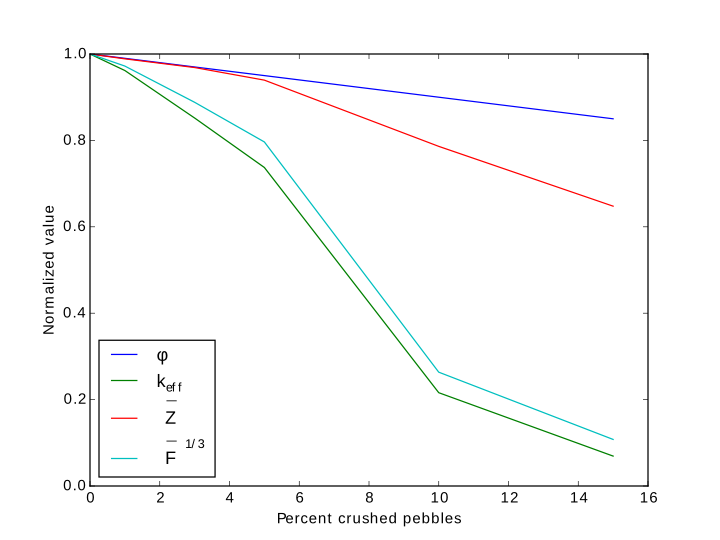
\includegraphics[width=\singleimagewidth]{figures/kEff_packingFraction}
    \caption{The normalized effective conductivity drops much more rapidly than the normalized packing fraction, $\phi$, while pebbles are crushed. The effective conductivity follows with reduced normal contact forces.}
\label{fig:packing-fraction}
\end{figure}

The large reduction in normal contact force (which leads to a large reduction in effective conductivity) is explainable based on the experimental setup of the numeric model. In the system, we had rigid walls in the $x$ and $z$ directions. These walls did not change after the substantial number of pebbles were crushed and removed. After the 15\% crushing event, the pebble bed appeared as \Cref{fig:15percent-crushed-pre}. A massive re-arrangement proceeds from the crushing event. As the pebble bed heats up, the thermal expansion of the pebbles is unconstrained as there exists an average gap of two pebble diameters in size above the pebbles to the top of the container. Numerically there is no limit to the pebble temperatures (phase change and sintering is not incorporated into the DEM calculations) so the pebbles heat and swell until coming into contact with the top wall, at which time they begin to press into one another (though lightly) to allow thermal conduction. The pebble bed after swelling is shown in \Cref{fig:15percent-crushed-swelling}.

\begin{figure}[!ht]
    \centering
    \begin{subfigure}[t]{\doubleimagewidth}
        \centering
        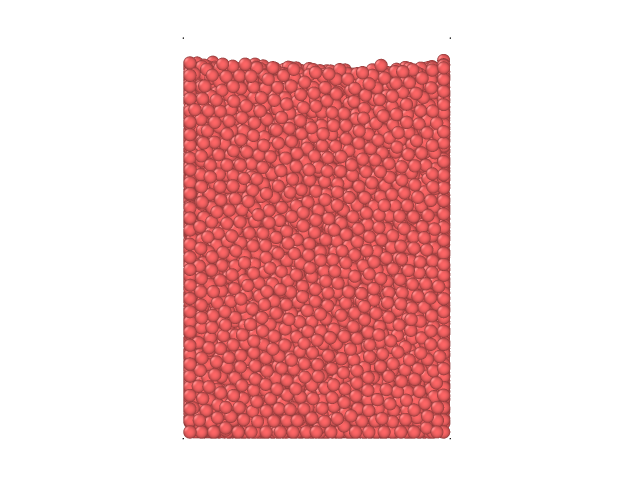
\includegraphics[width=\textwidth]{figures/heating_dte-02/15/0.15_pre_heat.png}
        \caption{Side-view of the pebble bed after resettling from the crushing event, before heating.}
        \label{fig:15percent-crushed-pre}
    \end{subfigure}
    \begin{subfigure}[t]{\doubleimagewidth}
        \centering
        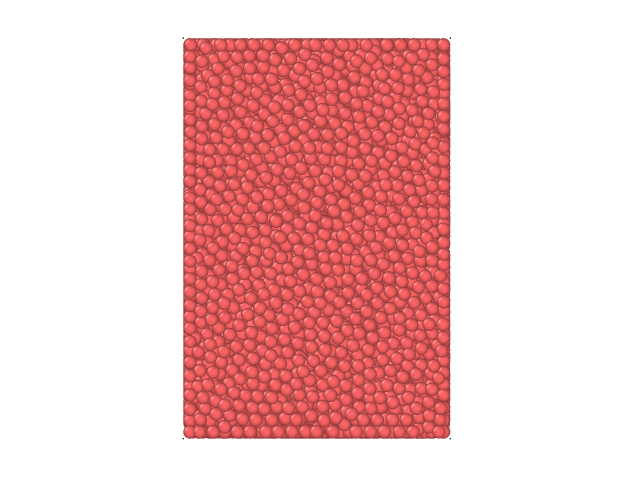
\includegraphics[width=\textwidth]{figures/heating_dte-02/15/0.15_post_heat.png}
        \caption{Side-view of the pebble bed after heating}
        \label{fig:15percent-crushed-swelling}
    \end{subfigure}
    \caption{In (a) we see the pebble bed after 15\% of the pebbles have been crushed (removed) and then after the heating cycle in (b). The gap formed after crushing is completely filled by swelling pebbles.}
\end{figure}

One last note that must be made concerning this study is on the initial packing state. As the first study performed with the new numeric tools, I was unaware of some of the measures of describing a pebble bed. For instance, I desired to match the experimental setup of our laboratory insomuch as matching general dimensions and packing fractions. What I did not realize, however, was that forcing the pebble bed to achieve a pre-determined packing fraction at the expense of ignoring initial inter-particle contact forces was improper. The error of this initial packing is immediately seen when comparing the $\keff$ of the baseline pebble bed with those of experiments, shown back in \Cref{fig:keff-pressure}. The pebble bed, in the absence of helium, ought to have had an effective thermal conductivity close to $\keff =$ \SI{0.2}{\watt\per\meter\per\kelvin}. What I found, however was an initial $\keff = $\SI{1.03}{\watt\per\meter\per\kelvin}. The initial average contact force in the pebble bed was approximately \SI{125}{N}, this value should have been seen as far too high from the outset.

Returning to this study, I attempted to assemble new pebble beds with different initial packing techniques. Instead of imitating the vibration-roof-pressing technique from the laboratory, or the overlap-relax technique used in this study, I created a second artificial packing technique. In this technique, the particles are all initially without contact friction and gravity was not initiated in the system. The limits of the periodic dimension were increased dramatically and the pebbles were allowed to fill the void space with large space between ($\phi \approx 0.10$). Then, slowly, the periodic boundaries shrunk which compressed the pebble bed. The frictionless, weightless pebbles were free to move around each other to create large packing fractions (up to $\phi = 64\%$) with minimal initial contact forces. These newly-packed pebble beds were again run to a thermal steady-state and an effective conductivity value established. In these cases, the initial $\keff$ was much closer to the values expected from physical experiments. The results of the contact forces in a number of new beds are given in \Cref{fig:contact-forces-scatter-initial}. The smaller initial contact forces lead to effective conductivities as shown in \Cref{fig:keff-initial}. If these new initial values of $\keff$ are compared to the damaged cases, the percent decrease in $\keff$ reported would be doubled. The results of these new packing techniques highlight the importance of the initial packing of the pebble bed when it comes to interpreting the output of the data. That is to say, neither of the results given are more correct or more incorrect than the other. They are simply more or less applicable to situations that have the same initial conditions -- including initial packing fraction and initial contact force.

\begin{figure}[!ht]
    \centering
    \begin{subfigure}[b]{0.4\textwidth}
        \centering
        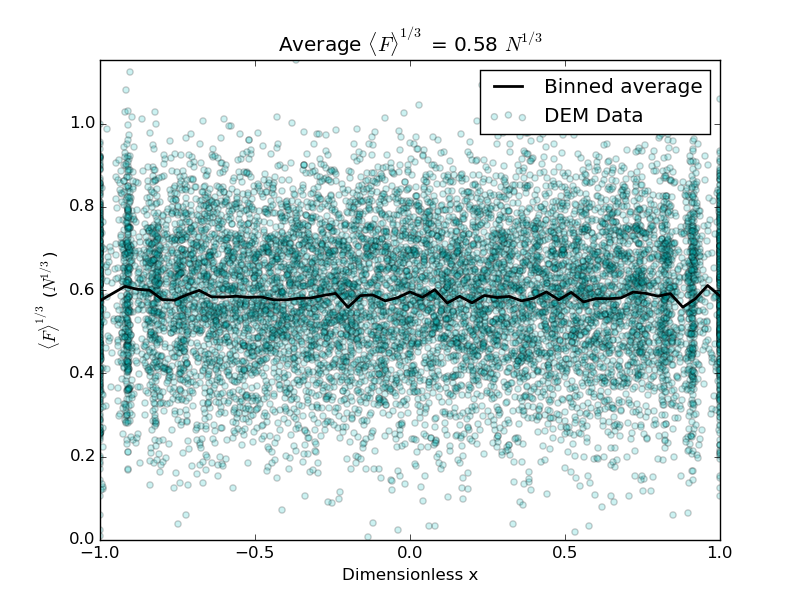
\includegraphics[width=\textwidth]{figures/initial_packing_study/62-deform-force-profile.png}
        \caption{Packed to $\phi = 62$\%}
    \end{subfigure}
    
    \begin{subfigure}[b]{0.4\textwidth}
        \centering
        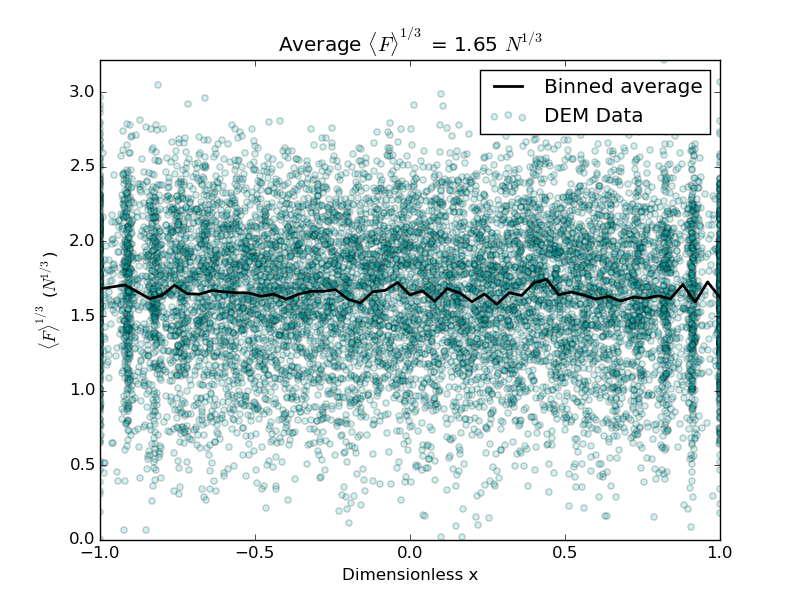
\includegraphics[width=\textwidth]{figures/initial_packing_study/63-deform-force-profile.png}
        \caption{Packed to $\phi = 63$\%}
    \end{subfigure}

    \begin{subfigure}[b]{0.4\textwidth}
        \centering
        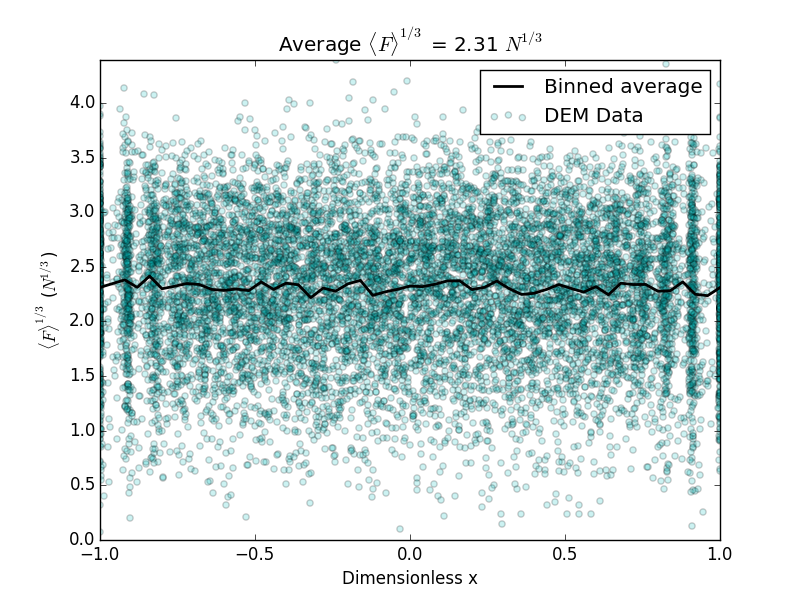
\includegraphics[width=\textwidth]{figures/initial_packing_study/64-deform-force-profile.png}
        \caption{Packed to $\phi = 64$\%}
    \end{subfigure}
    \caption{Initial force distributions in pebble beds packed with a new routine.}
\label{fig:contact-forces-scatter-initial}
\end{figure}

\begin{figure}[!ht]
    \centering
    \begin{subfigure}[b]{0.4\textwidth}
        \centering
        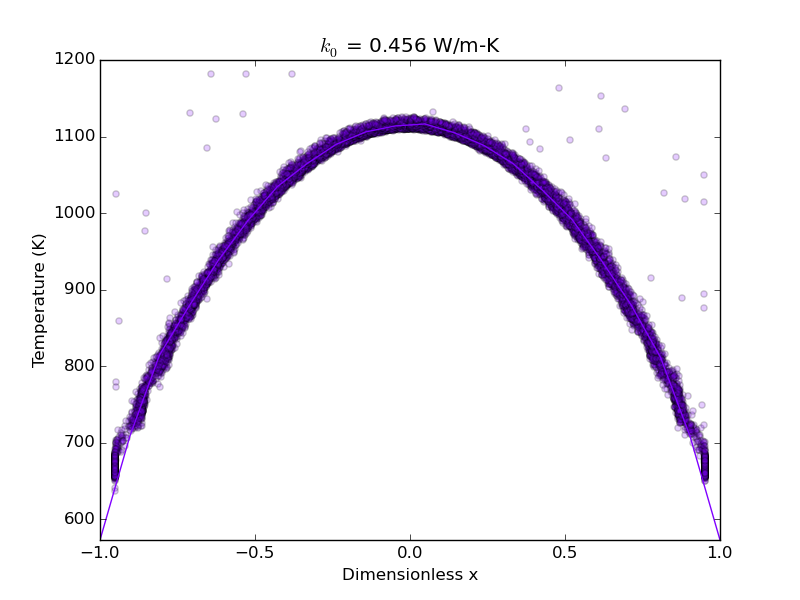
\includegraphics[width=\textwidth]{figures/initial_packing_study/62percent-deform-packing.png}
        \caption{Packed to $\phi = 62\%$}
    \end{subfigure}
    
    \begin{subfigure}[b]{0.4\textwidth}
        \centering
        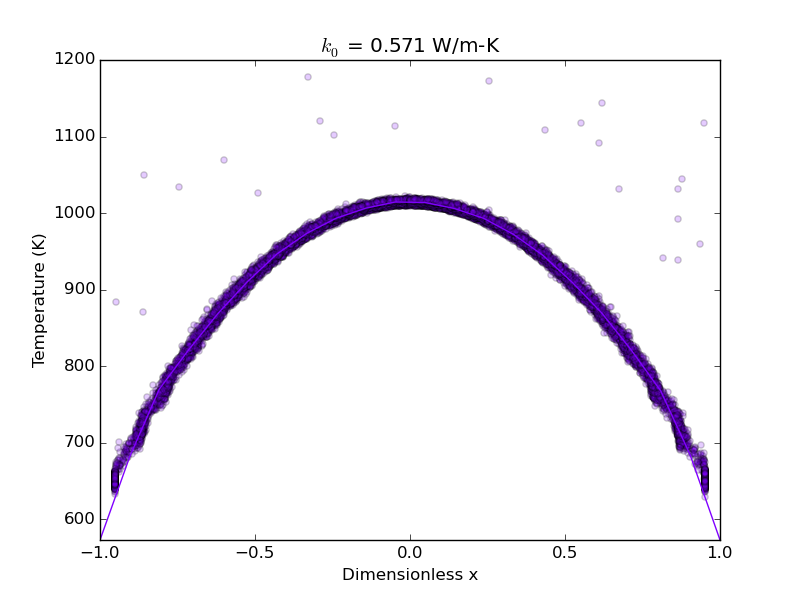
\includegraphics[width=\textwidth]{figures/initial_packing_study/63percent-deform-packing.png}
        \caption{Packed to $\phi = 63\%$}
    \end{subfigure}

    \begin{subfigure}[b]{0.4\textwidth}
        \centering
        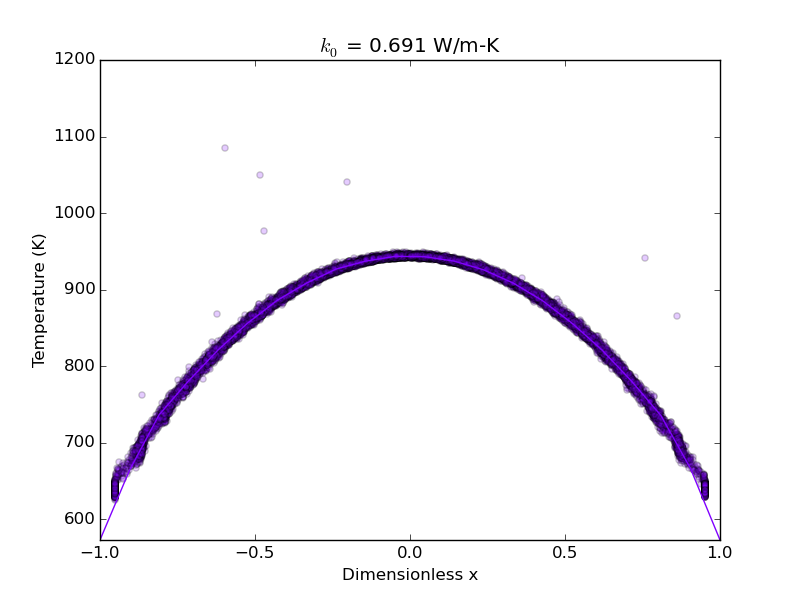
\includegraphics[width=\textwidth]{figures/initial_packing_study/64percent-deform-packing.png}
        \caption{Packed to $\phi = 64\%$}
    \end{subfigure}
    \caption{Initial $\keff$ in the lightly-packed pebble beds are much closer to values measured in experiments in vacuum.}
\label{fig:keff-initial}
\end{figure}





\FloatBarrier



\subsection{Conclusions}
\label{sec:dem-conclusions}
This first study established the power of DEM modeling and its use as a foundation for the later studies with augmentations of helium flow. I simulated a pebble bed with a specified fraction of the pebbles crushed during operation, then determined the repercussions of the missing pebbles as they affect the macroscopic property of effective thermal conductivity. I used the assumption of homogeneous, random locations of pebble failure to induce a failure routine without requiring external loads on the bed to actually induce the pebble crushing. After heating to a steady-state, an effective thermal conductivity was calculated for the pebble bed. The results show that large amounts of pebble failure correspond to large decreases in the conductive transport of energy through the pebble bed. The increase was due almost exclusively to a drop in the inter-particle forces which lead to a large increase in temperature differences between neighboring pebbles.

As the first step in the modeling effort, there were many simplifications that had to be made. I will explain here the shortcomings of the assumptions and simplifications of this study before drawing any major conclusions from the results.

First, the `container walls' surrounding the pebble bed in this model are completely rigid and do not react as the swelling pebble bed presses into them while heating. The confined thermal expansion leads to higher contact forces in the pebble bed than what may exist in reality. Furthermore, as pointed out in the results, the initial contact force is strongly dependent on the \textit{initial packing state} and the contact forces are the greatest determining factor in $\keff$ for a bed. The initial packing state of the bed in this study gave abnormally high initial contact forces and thus abnormally high initiall $\keff$. A different packing scheme was shown to result in the same initial packing fraction but with greatly reduced initial contact forces; this packing technique will be used in future models. 

Second, we saw from Fig.\ref{fig:temp-scatters} that the majority of the pebbles in the ensemble have their temperatures close fitting to an average curve but a number of the pebbles had less thermal contact with neighboring particles and consequently had much larger temperatures. This was true even in the baseline case of a tightly packed ($\phi =$\num{0.64}) pebble bed. This phenomena is possible because the contribution to heat transfer of the interstitial gas was not considered in this model and the flowing helium gas is expected to prevent any runaway temperatures of individual pebbles as it provides another route of energy transfer in the bed. This will be addressed in \cref{sec:cfd-dem-studies}.

Lastly, the pebble crushing did not conserve mass between pre- and post-crushing in the pebble beds. This is an issue we address in the fragmentation study of \cref{sec:fragmentation}. There was also no predictive tool used to determine when pebbles would crush based on their inter-particle contact forces. I simply allowed an arbitrary number of pebbles to remove from the system. A predictive tool may not have expected even 2\% of the pebbles to be damaged, much less the 15\% to which I pushed the pebble bed. The predictive tool is discussed in \cref{sec:failure-study} and will be applied to later models.

In spite of the limitations mentioned, it is still worth drawing conclusions from the results of this study. The results shown in Figs.~\ref{fig:contact-forces-scatter} and~\ref{fig:coord-scatter} demonstrate that the heat transfer through a pebble bed is simultaneously a function of both the coordination number and inter-particle contact forces. The average values of both of these parameters reduced as pebbles in the bed were crushed. But by far the most important factor appears to be the inter-particle contact force. Between the baseline case and the bed with 15\% damage, the average inter-particle forces drop by an entire order of magnitude. The $\keff$ follow suit with a decrease to 10\% of the original value. Interestingly, when a pebble bed has lower overall inter-particle contact forces such as what we see when pebbles are crushed, we would predict fewer pebbles are likely to break. This result implies that pebble breakage is self-dampening; as pebbles begin to break the ensemble quickly relaxes and avoids future pebble failure. So while in this study we induced failure up to $\eta = 15\%$ without a concern for predicting if such a large amount would break, such large values may not occur in real beds during operation of a fusion reactor. 

The most important conclusion to draw from the this DEM study is simply the usefulness of the DEM tools for opening a window into the micro-mechanical world of the pebble bed. The transient DEM simulations allowed us to explore the evolving packing structure and the manifestation of the packings into macroscopic properties such as the effective thermal conductivity. The DEM simulations revealed that some of the most negative effects nervously anticipated in the solid breeder did not emerge: bed detachment from the walls and bridge-jamming of regions to isolate groups of pebbles from heat transfer paths. There remain some features which must be addressed, but the DEM approach used in this dissertation has demonstrated its value as a tool for solid breeder designers. 














%%%%%%%%%%%%%%%%%%%%%%%%%%%%%%%%%%%%%%%%%%%%%%%%%%%%%%%%%%%%%%%%%%%%%%%%%%%%%%%%%%%%%%%%%%%%%%
\section{Dynamically coupled CFD-DEM Study on Effective Conductivity of Pebble Peds with Pebble Damage}\label{sec:cfd-dem-studies}

In this section I demonstrate the transient coupling between DEM models of particle conductive heat transfer and inter-particle contact forces with the helium models of volume-averaged conservation equations. Thermal models of the pebble beds of solid breeders for fusion reactors are incomplete without consideration of the helium purge gas and its interaction with the poorly conductive porous network of pebbles. The simulation setup, material parameters, results and important conclusions will be discussed.
\subsection{Modeling Setup, Boundary Conditions, and Coupling}\label{sec:cfd-dem-setup}
For this simulation, I begin with the same well-packed pebble bed set up in \cref{sec:dem-studies-effective-conductivity}. I will analyze a full-packed bed and a damaged bed with $\eta = 10$\% of broken pebbles. The random removal technique of inducing `damage' to the bed was again used (in the same manner as described in \cref{sec:dem-studies-effective-conductivity}). The intent is to deduce changes in thermophysical properties when helium is considered in the thermal transport network of the pebble bed -- and as a function of the morphological changes due to damaged pebbles.

The domain of the pebble bed in this study is a clone of the DEM study done previously. The fluid domain is constructed to include an inlet and outlet region of fluid to permit development of the flow profiles. The inlet region is 5 pebble diameters in length and the outlet is 30 pebble diameters. No-slip boundary conditions are enforced at the walls at the $x$-limits of the region. To match the DEM domain, periodic boundary conditions are used in the $y$-limits. The inlet face of the fluid is specified at a constant $\vec{v} = (5, 0, 0)$ \si{\centi\meter\per\second}. The outlet face is specified with OpenFOAM's `inletOutlet' command with a given pressure. This boundary condition allows the inlet pressure to float to value that satisfies the specified inlet velocity and outlet pressure. The temperature is specified as a constant $T_w = $ \SI{573}{\kelvin} at the $x$-walls as well as the inlet. The outlet condition of the temperature field is similarly given to be `inletOutlet' with OpenFOAM.

The size of the CFD cells were chosen to be large enough to fit approximately 5 pebbles, for which the divided technique of computing void fraction is applicable (see \cref{sec:lag-eul-mapping}); the ratio of cell volume to particle volume was $V_\text{cell} / V_p = 7.46$. The helium, in this first model, was modeled with constant fluid properties. The values are given in Table~\ref{tab:cfd-properties}.

The Koch-Hill-Ladd drag model is employed in the style of Model B with an Archimedes pressure for buoyancy term. The terminology of these CFD coupling drag models is discussed in Ref.~\cite{Zhou2010} The Nusselt number correlation of Li \& Mason is used for calculating the Nusselt number. OpenFOAM's dummy turbulence model (which is nothing more than a laminar model) is used.

An implicit time marching scheme is employed with a time step in the fluid domain of $\Delta t_f =$\SI{1e-4}{\second}. The small time step is not necessary to capture the fluid flow. The momentum equation is essentially not even transient as a steady-state laminar solution is achieved almost instantaneously in comparison to the long time span required to reach thermal steady state. The small time step is necessary for a relatively tight coupling to the pebble bed as the temperatures increase on the pebbles. Integration schemes of gradients, divergence terms, and laplacians are all Gauss linear or Gauss limitedLinear (as defined in OpenFOAM). The time step of the DEM is $\Delta t_s =$ \SI{1e-7}{\second} which must be small for stability of the DEM explicit integration. The coupling between CFD and DEM domains occurs every 10 time steps of the fluid domain - equating to every \num{10000} in the pebble domain.

The layout of the pebble bed inside the CFD domain is shown in Figs.~\ref{fig:cfdem-domain-x}, \ref{fig:cfdem-domain-y}, and~\ref{fig:cfdem-domain-z}. Notable of the layout is the relaxation of the mesh size in the direction of the periodic boundaries. The size is permitted as there are few variations in fluid or temperature in the periodic direction. The meshes are made much smaller in the direction between cooling boundaries. In this direction ($x$-direction), we need the meshes small enough to resolve a temperature and velocity profiles across the bed between centerline and cooling boundaries. We also want to capture the behavior of near-wall arrangement of the pebble bed. 

\begin {table}[htp] %
\caption{Constant fluid properties of helium purge gas in CFD-DEM coupling.}
\label {tab:cfd-properties} \centering %
\begin {tabular}{ ccccc }
\toprule %
$\nu$				&	$\alpha$				&	$k$		&	$C_p$		& $\rho$		\\
(\si{\meter\squared\per\second})			&	(\si{\meter\squared\per\second})				&	(\si{\watt\per\meter\per\kelvin})	&	(\si{\joule\per\kilogram\per\kelvin})	& (\si{\kilogram\per\cubic\meter})	\\\toprule
\num{4.02e-4} &	\num{6.06e-4}	& 	\num{0.2}		& 	\num{5192.8}		& 	\num{0.175}		\\\bottomrule
\end{tabular}
\end{table}


\begin{figure}[t]
	\centering
	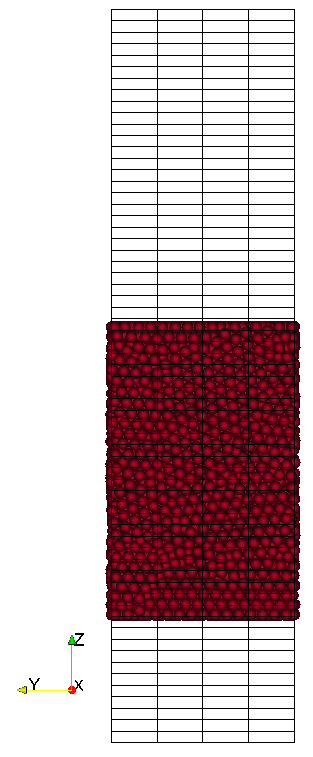
\includegraphics[width=0.4\textwidth]{figures/x-side-view}
    \caption{Side view of the pebble bed as it resides in the CFD mesh. The meshes in the direction of the periodic faces are allowed to be larger than others.}\label{fig:cfdem-domain-x}
\end{figure}

\begin{figure}[t]
	\centering
	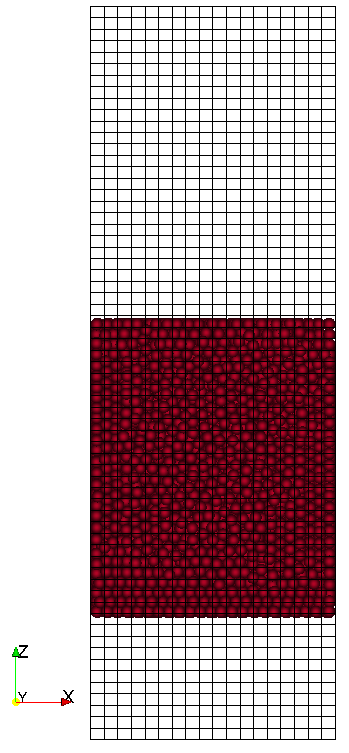
\includegraphics[width=0.4\textwidth]{figures/y-side-view}
    \caption{Front view of the pebble bed as it resides in the CFD mesh. The meshes in the direction of cooling are chosen to be large enough to fit many pebbles but small enough to provide a resolved temperature profile.}\label{fig:cfdem-domain-y}
\end{figure}

\begin{figure}[t]
	\centering
	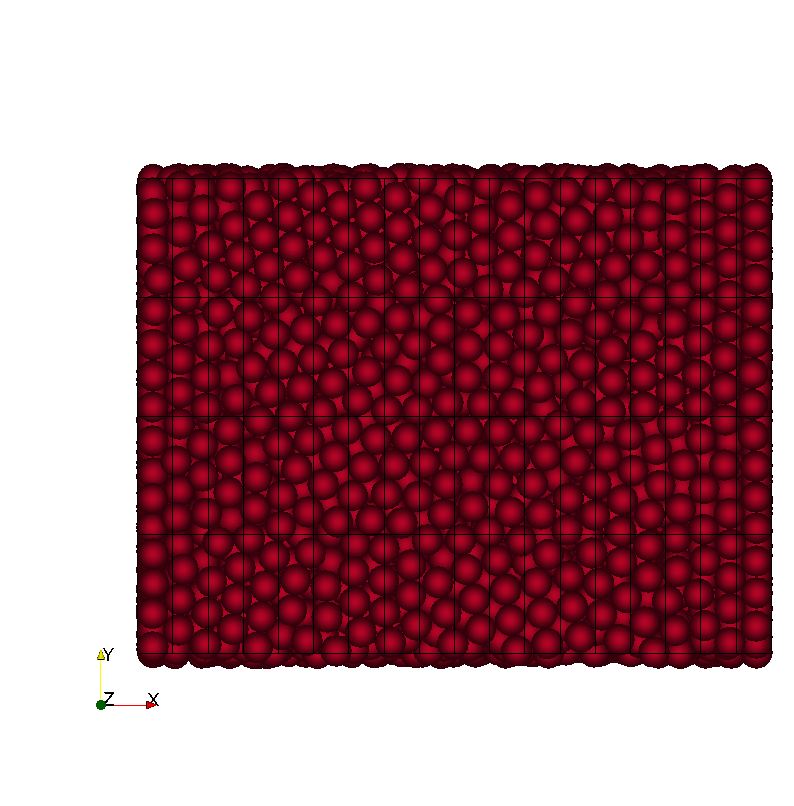
\includegraphics[width=\singleimagewidth]{figures/z-top-view}
    \caption{Top view of the pebble bed as it resides in the CFD mesh.}\label{fig:cfdem-domain-z}
\end{figure}


While the energy transport is the main concern of the pebble bed, I perform a simple validation of the CFD-DEM routine against known pressure-drop correlations to provide confidence in the overall coupling and volume-averaging technique. After pressure drop is shown to be consistent with empirical predictions, I proceed with the thermal analysis.
\FloatBarrier


\subsection{Pressure Drop}

The CFD-DEM coupling was run at various particle Reynolds numbers and the overall pressure drop of the packed bed was measured. The pressure drop is compared against the well-known Kozeny-Carman and Ergun equations. The Kozeny-Carman is known to fit better with experimental data at very small Reynolds numbers while the Ergun equation is a more general equation meant to span a large range of Reynolds numbers. In \Cref{fig:cfdem-pressure-drop} we see the CFD-DEM coupling model is providing bed-scale pressure drops that match very well with Kozeny-Carman over the Reynold’s numbers applicable to helium purge flow in fusion reactors ($\Re_p \approx 1$). 

Seki\etal experimentally studied the flow of helium purge gas in efforts to better understand tritium recovery.\cite{Seki2013a} They ran a representative volume of pebbles up to flow rates of \SI{100}{\liter\per\minute} and also found that Ergun's pressure drop prediction was highly accurate for the pebble beds as long as the viscous contribution (see the right-most term in \Cref{eq:ergun-pressure}) was small, \textit{e.g.} when the Reynolds number of the packed bed is small. This result is a strong validation of the macroscopic results of pressure drop as calculated by the CFD-DEM simulation of a packed bed.

\begin{figure}
        \centering
        \begin{subfigure}[b]{0.7\textwidth}
                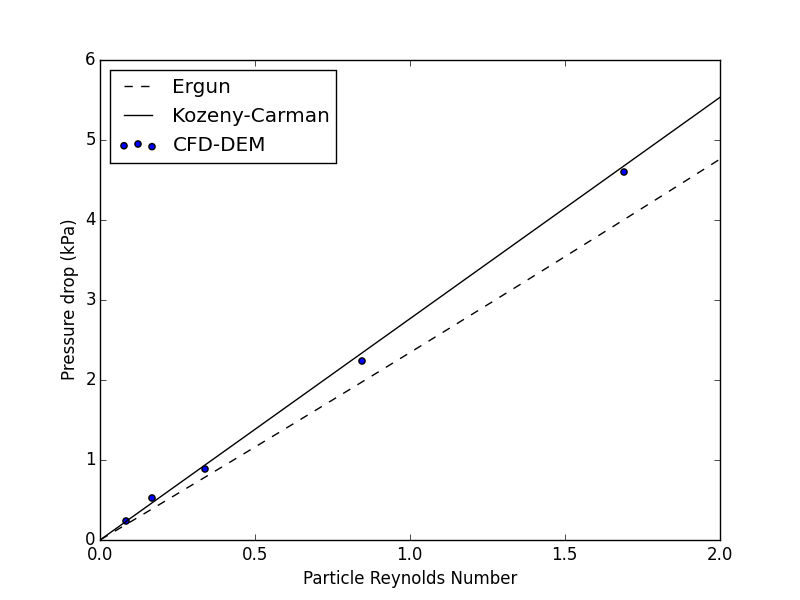
\includegraphics[width=\textwidth]{figures/pressureDrops-full.png}
                \caption{Well-packed bed}
                \label{fig:pressure-drop-full}
        \end{subfigure}%
        
          %add desired spacing between images, e. g. ~, \quad, \qquad, \hfill etc.
          %(or a blank line to force the subfigure onto a new line)
        \begin{subfigure}[b]{0.7\textwidth}
                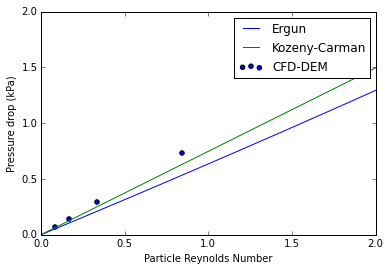
\includegraphics[width=\textwidth]{figures/pressureDrops-evap.png}
                \caption{Re-settled bed}
                \label{fig:pressure-drop-evap}
        \end{subfigure}
        \caption{Pressure drop calculations across packed beds, solved by CFD-DEM, fit well to the Kozeny-Carman empirical relation.}\label{fig:cfdem-pressure-drop}
\end{figure}



\subsection{Effective Thermal Conductivity from CFD-DEM}\label{sec:cfd-dem-effective-conductivity}

The simulation is allowed to run to thermal steady-state with nuclear heating and wall cooling. After reaching a steady solution, I analyze the temperature profiles of the fluid and pebble bed. The temperature of the fluid volume from the simulation of the well-packed bed is shown in \Cref{fig:cfdem-complete-domain}. The flow field is also visualized in \Cref{fig:cfdem-streamlines}; in this figure the pebble bed is clipped at the centerline to allow viewing of the helium streamlines. Apparent in the figure is temperature profiles in the helium from centerline to wall that qualitatively mirror temperature profiles in the pebble bed. The two beds in our system, well-packed and resettled, were run to thermal steady-state with nuclear heating and wall cooling in both pure DEM and coupled CFD-DEM simulations for comparison. From steady-state temperature distributions, seen in the pebble scatter plots in \Cref{fig:cfdem-x-T}, an average profile is calculated and an effective thermal conductivity computed following the procedure shown in \cref{sec:keff-analogy}. The values are tabulated in Table~\ref{tab:cfdem-keff}. 

In the case of pure DEM, energy is transported solely along conduction routes in the ensemble. When the packing of the bed is disturbed, this results in a substantial drop in effective conductivity (a drop of 31\%). Perhaps more important than the reduction in effective conductivity, is the growth in number of isolated rattlers. Because heat deposition is volumetrically applied, pebbles with poor conduction routes become much hotter than their neighbors. This is evident in the high temperatures seen in many of the pebbles in the \Cref{fig:x-T-evap}. Over-heating of isolated pebbles could induce sintering and impact their tritium release even when the average temperatures measured in the bed are well below sintering values.

When CFD-DEM beds are analyzed, there is still a large reduction in effective conductivity (22\% drop), but interesting to note is the lack of high temperature rattlers. In the CFD-DEM scatter plot of \Cref{fig:x-T-evap}, there is evidence of the reduced heat transfer in the same region as the isolated pebbles from the DEM bed, but the temperatures are much closer to the average values of neighboring pebbles. The helium purge gas has locally smoothed out the temperatures and provided heat transport paths for pebbles that have loose physical contact with neighbors.

In spite of the 22\% decrease in effective conductivity, the maximum temperature of the pebble bed only increased 6.2\% (from \SIlist{725;751}{\kelvin} when helium is included in the model. This result is significant for solid breeder designers. They may choose a solid breeder volume such that in the event of extensive pebble cracking, the maximum temperature of the bed would remain within the ideal windows dictate for the lithium ceramics.

An accompanying result is the increased amount of energy carried out of the system by the helium purge gas. In Table I, the last column provides the ratio of energy carried out of the system to the nuclear energy deposited into the bed. The amount of energy carried out by the helium increased from \numlist{1.15;1.52}\% from the well-packed to damaged beds.

\begin{figure}[t]
    \centering
    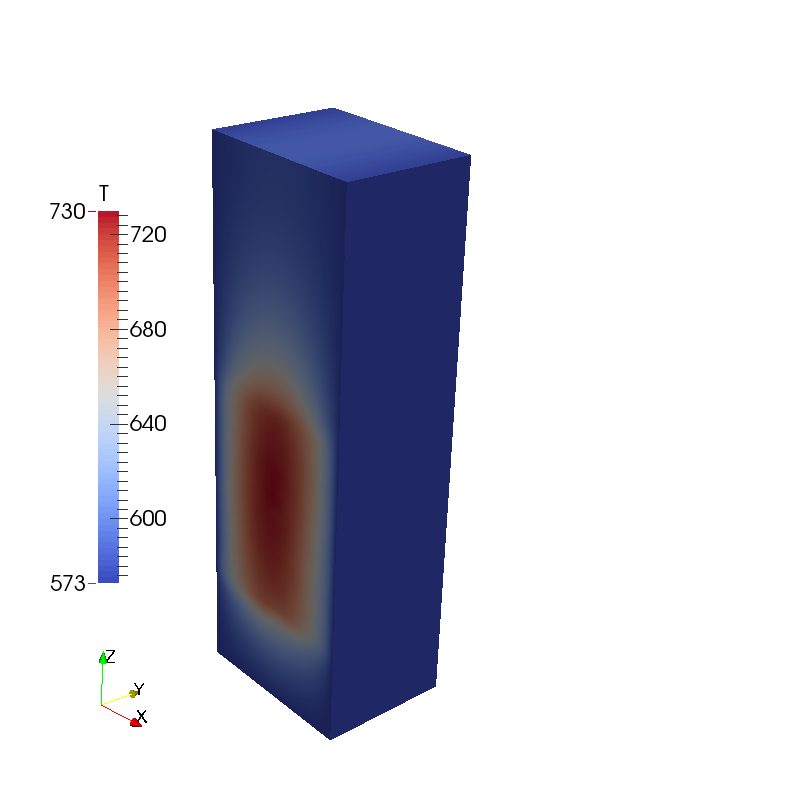
\includegraphics[width=\singleimagewidth]{figures/full-cfd-dem-fluid-temp}
    \caption{View of the complete fluid domain at thermal steady state.}\label{fig:cfdem-complete-domain}
\end{figure}


\begin{figure}[t]
    \centering
    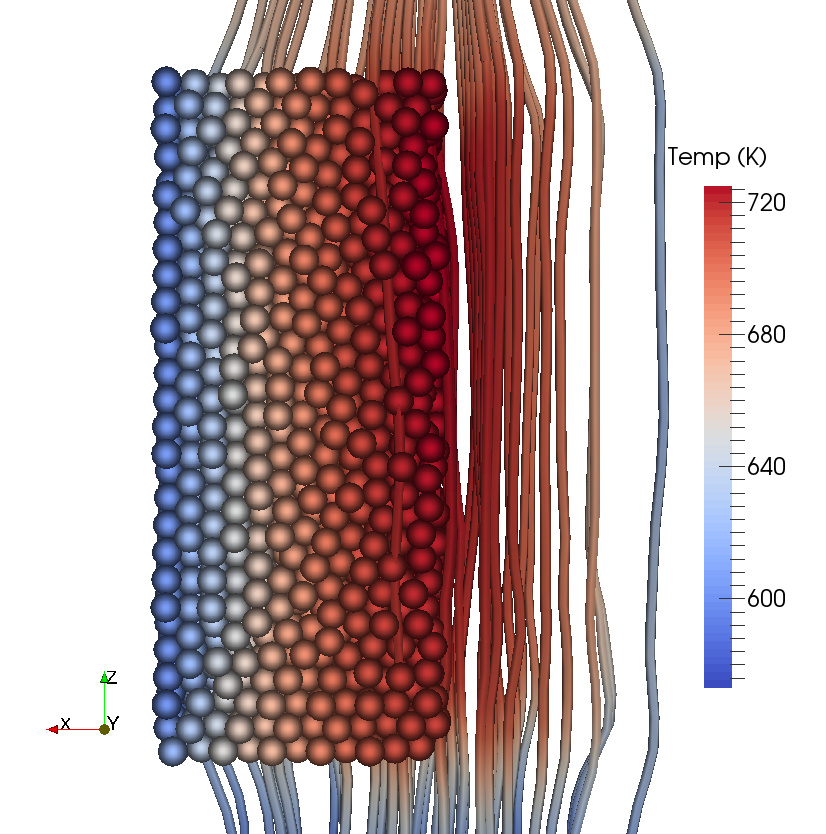
\includegraphics[width=\singleimagewidth]{figures/cfd-dem-streamlines2}
    \caption{Cut-away view of the pebble bed with streamlines of helium moving in generally straight paths from inlet to exit.}\label{fig:cfdem-streamlines}
\end{figure}


\begin{figure}
        \centering
        \begin{subfigure}[b]{0.5\textwidth}
                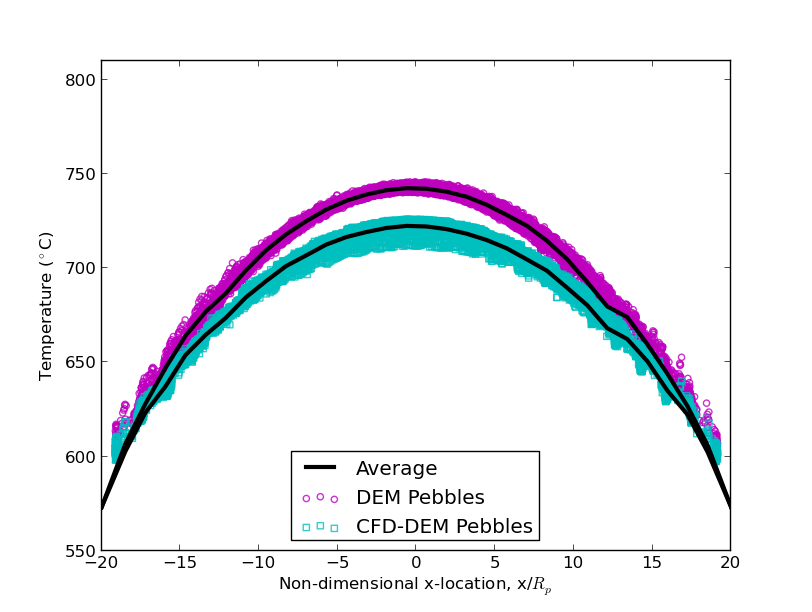
\includegraphics[width=\textwidth]{figures/full-x-T-color}
                \caption{Well-packed bed}
                \label{fig:x-T-full}
        \end{subfigure}%
        
          %add desired spacing between images, e. g. ~, \quad, \qquad, \hfill etc.
          %(or a blank line to force the subfigure onto a new line)
        \begin{subfigure}[b]{0.5\textwidth}
                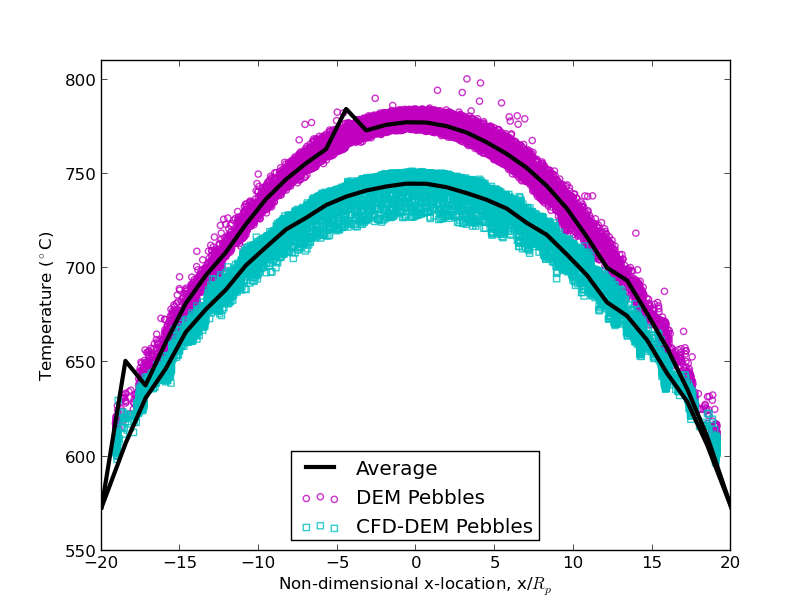
\includegraphics[width=\textwidth]{figures/evap-x-T-color}
                \caption{Re-settled bed}
                \label{fig:x-T-evap}
        \end{subfigure}
        \caption{Scatter temperature profiles of pebbles in a bed that is: well-packed (left) and resettled after 10\% of pebbles were removed from crushing (right). The introduction of helium into the simulation contributes to both lower overall temperatures (higher effective conductivity) and the smoothing out of high temperatures of isolated pebbles.}\label{fig:cfdem-x-T}
\end{figure}



\begin {table}[htp] %
\caption{Pebble bed values from the test matrix of the beds analyzed in this study.}
\label {tab:cfdem-keff} \centering %
\begin {tabular}{ rccccc }
\toprule %
			& 	\multicolumn{2}{c}{$\keff$}	&   \multicolumn{2}{c}{$T_\text{max}$}	&	$\frac{Q_h}{Q_\text{nuc}}$		\\
			& 	\multicolumn{2}{c}{(\si{\watt\per\meter\per\kelvin})}			&	\multicolumn{2}{c}{(\si{\kelvin})}				&									\\
			& 	DEM 		& 	CFD-DEM				&	DEM 		& 	CFD-DEM 			& 	CFD-DEM							\\\toprule
Well-packed	& 	0.96		& 	1.09				& 	745			& 	725					& 	1.15							\\
Resettled	& 	0.66		& 	0.85				& 	800			& 	751					& 	1.52							\\\bottomrule
\end{tabular}
\end{table}





\FloatBarrier



\subsection{Conclusions}

In this study I extended the thermophysical analysis of damaged pebble beds begun in \cref{sec:dem-studies} to include the influence of helium in a volume-average sense. This study grew from the prior one and the pebble bed representation of damage suffered all the same limitations mentioned in the closing of the last study, they will not be mentioned again here for the sake of brevity.

The CFD-DEM approach was validated, at least in terms of the volume-averaged Navier-Stokes equations, with a parametric study of pressure drop as a function of Reynolds number. When helium flowed over the DEM pebble beds, the pressure drop fit well to the well-established Kozeny-Carman correlation.

Two representative pebble beds, one well-packed and one with 10\% damaged pebbles, were run to thermal steady state with nuclear heating and cooling at a pair of walls.  The pair of pebble beds were considered with only conduction heat transfer of DEM and also with the helium enhancements to heat transfer with CFD-DEM. In the DEM beds, we saw that there always exist hot rattlers in pebble beds -- even well-packed ones. These pebbles heat from the volumetric source but have no outlet for the energy as their contacts with neighbors are very light. However, with the inclusion of helium flow eliminated the hot rattlers from both pebble beds analyzed.

When comparing the impact of pebble damage with and without the modeling of helium, the models including helium showed less of an impact on reduced effective thermal conductivity when the bed experienced the extensive 10\% damage of pebbles. Furthermore, the maximum bed temperature increased less due to pebble damage when helium was included, when compared to DEM-only beds.

This study is a useful demonstration of the power of the dynamically coupled CFD-DEM approach. The DEM simulation was capable of continually monitoring inter-particle forces and individual particle temperatures such that any of the crush-prediction, fragmentation, and thermal expansion methods developed in this dissertation can continue to transiently alter the morphology of the pebble bed. Meanwhile, the volume-averaged approach to conservation equations of the fluid allow for an efficient overlaying of the fluid contribution to the thermophysical behavior of the pebble bed.

There are simplifications to the fluid flow and its impact on the thermal transport in the pebble bed that are made in the volume-averaging technique. The simplifications may mask some important physical features of the flow and energy fields but nevertheless provide valuable information on the pebble bed in an efficient manner and should continue to be developed for solid breeder research.











\section{Temperature Distributions with Breeder Orientation, Pebble Fragmentation}\label{sec:isfnt-12}


\subsection{Introduction}

We apply coupled computational fluid dynamics and discrete element method (CFD-DEM) modeling tools with new numerical implementations of pebble fragmentation to study the combined effects of granular crushing and ensemble restructuring, granular fragment size, and initial packing for different breeder volume configurations. In typical solid breeder modules, heat removal from beds relies on maintaining pebble-pebble and pebble-wall contact integrity. However, contact is disrupted when an ensemble responds to individually-crushed pebbles. Furthermore, restructuring of metastable packings after crushing events are, in part, dependent on gravity forces acting upon the pebbles. We investigate two representative pebble bed configurations under constant volumetric heat sources; modeling heat removed from beds via inter-particle conduction, purge gas convection, and contact between pebble beds and containers. In one configuration, heat is removed from at walls oriented parallel to the gravity vector (no gap formation possible); in the second, heat is removed at walls perpendicular to gravity, allowing for the possibility of gap formation between bed and wall. Judging beds on increase in maximum temperatures as a function of crushed pebble amount, we find that both pebble bed configurations to have advantageous features that manifest at different stages of pebble crushing. However, all configurations benefit from achieving high initial packing fractions.



\subsubsection{Simulation domain, boundary conditions, and material properties}

Two ITER-relevant volumes are considered in this study, sketched in \Cref{fig:x-domain,fig:y-domain}. They are differentiated from each other by gravity's direction in the configuration. Because of their similarity, we use generic coordinate systems $(\chi, \zeta)$. Thus $\chi$-configurations, shown in \Cref{fig:x-domain}, have $\chi = y$ and $\zeta = x$ while $\zeta$-configurations, \Cref{fig:y-domain}, have $\chi = x$ and $\zeta = y$. The $\zeta$-configuration in this study is meant to represent the orientation of European Union's TBM \cite{Hernandez2013}, while the $\chi$ configuration is an orientation adopted by many other current TBM designs in ITER \cite{Cho2008,Feng2012a}.

\begin{figure}[!ht]
    \centering
    \begin{subfigure}[b]{0.44\textwidth}
        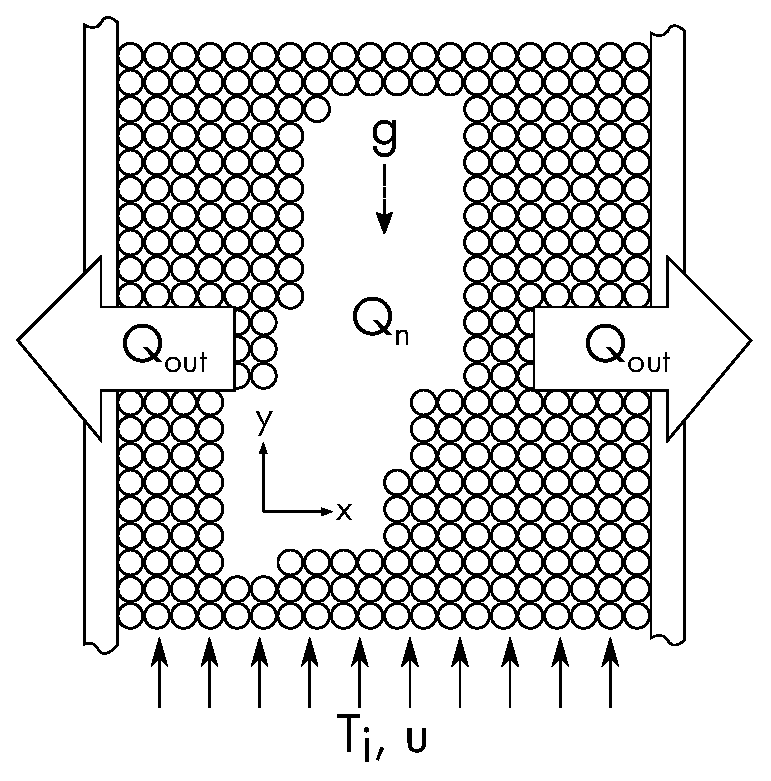
\includegraphics[width = \textwidth]{figures/x-domain.eps}
        \caption{$\chi$-configuration: heat removed in the $x$-direction.}\label{fig:x-domain}
    \end{subfigure}
    ~
    \begin{subfigure}[b]{0.44\textwidth}
        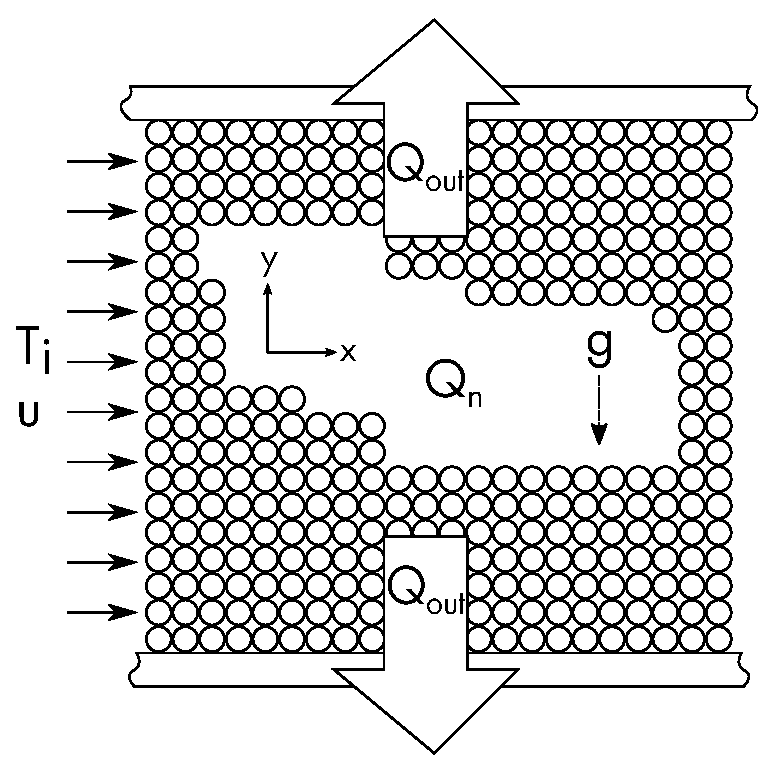
\includegraphics[width = \textwidth]{figures/y-domain.eps}
        \caption{$\zeta$-configuration: heat removed in the $y$-direction}\label{fig:y-domain}
    \end{subfigure}
    \caption{Sketches of the two breeder orientations show that gravity settling will not allow gaps between pebbles and walls in the $\chi$-configuration. However for the $\zeta$-configuration, gravity-induced resettling can create a gap between pebbles and upper wall. }\label{fig:domains}
\end{figure}

In terms of the generic coordinates, outflow of bed heat to coolant is along $\zeta$. Constant temperature boundaries, $T_w$, exist at the edges of that dimension. As sketched in \Cref{fig:domains}, gravity resettling in the $\chi$ configuration will not allow gap formation between bed and wall. However, in the $\zeta$-config it is possible for a gap to form between top coolant walls and pebbles after gravity resettling. A constant nuclear heat rate was applied to every particle in the bed which is representative of the highest source term anticipated in current ITER designs of solid breeder blankets, $q''' = $~\SI{8e6}{\watt\per\meter\cubed}.

The simulation consists of pebbles of diameter $d_p = $~\SI{1}{\milli\meter}, in beds filled to two initial packing fractions, $\phi_{1,2} = 62, 64\%$. Mechanical properties of the pebbles are given in \Cref{tab:peb-props}. To note is the Young's modulus chosen for pebbles in this study. In a past experimental study, Van Lew \textit{et al}. found that individual pebbles behaved in a manner indicative of having a Young's modulus from 20 to 60\% of values reported in literature for sintered blocks of \lit~and \lis~\cite{VanLew2015a}. Therefore to maintain some generality to this study, we have chosen a Young's modulus at a nominal value of $E=$~\SI{60}{\giga\pascal} to generically represent either ceramic pebble.

Pebble bed widths in $\zeta$ are \SI{20}{\milli\meter}, a size comparable to breeding volumes of many ITER TBM designs \cite{Hernandez2013,Cho2008,Feng2012a}. Bed depths (in the $z$-direction, in/out of the page in \Cref{fig:x-domain,fig:y-domain}) are \SI{5}{\milli\meter}, with periodic boundary conditions. Bed lengths in $\chi$ vary to accommodate \SI{6000} pebbles, initially, with given initial packing fractions; the length is approximately \SI{50}{\milli\meter}. Virtual walls are placed at extents of $\chi$ and $\zeta$ dimensions. Walls in $\zeta$ had constant temperature boundaries of $T_{w,s}$, all walls have mechanical and thermal properties of structural steel, given in \Cref{tab:wall-props}.

Fluid domains, overlaid on DEM pebbles, have fluid inlet and outlet regions of lengths \SI{10}{\milli\meter} and approximately \SI{51}{\milli\meter}, respectively. The side walls of the fluid domain were adiabatic in inlet and outlet regions and had constant temperature boundaries where they contacted the pebble bed, $T_{w,f}$. Fluid entered with a constant velocity magnitude of \SI{5}{\centi\meter\per\second} and constant temperature $T_i$. At present, temperature-dependencies of helium properties have not been incorporated into the model. Over the range of \SIrange{400}{900}{\celsius}, increases in helium momentum and thermal diffusivities are both essentially linear and thus an arithmetic mean for properties over that range is used as a first approximation. Future models will incorporate temperature-dependence of fluid properties. Fluid transport properties are given in \Cref{tab:fluid-props}. 
%---------------------------------------------------------------------------------------
% FIGURES
%---------------------------------------------------------------------------------------
% \begin{figure*}[!ht]
%        \centering
%        \begin{subfigure}[b]{0.45\textwidth}
%                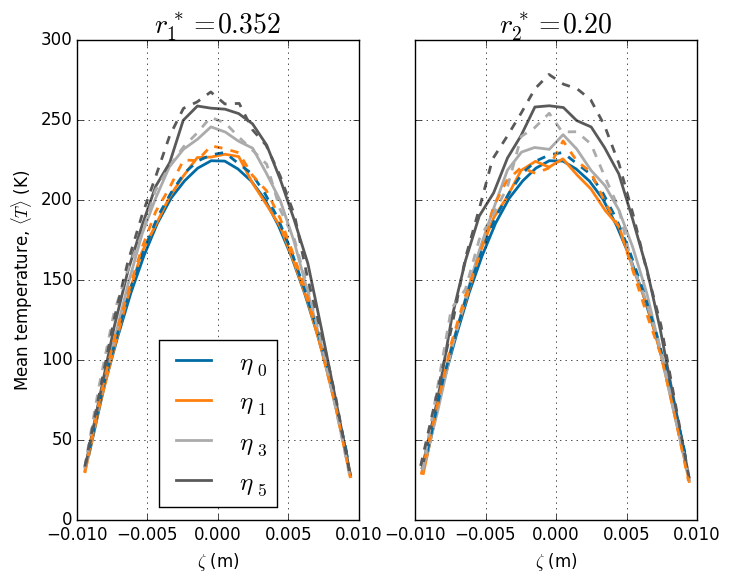
\includegraphics[width=\textwidth]{figures/62-percent-T-profiles.png}
%                \caption{Initial packing fraction of $\phi_1 = 0.62$.}
%                \label{fig:62-T-profile}
%        \end{subfigure}%
%        ~ %add desired spacing between images, e. g. ~, \quad, \qquad, \hfill etc.
%          %(or a blank line to force the subfigure onto a new line)
%        \begin{subfigure}[b]{0.45\textwidth}
%                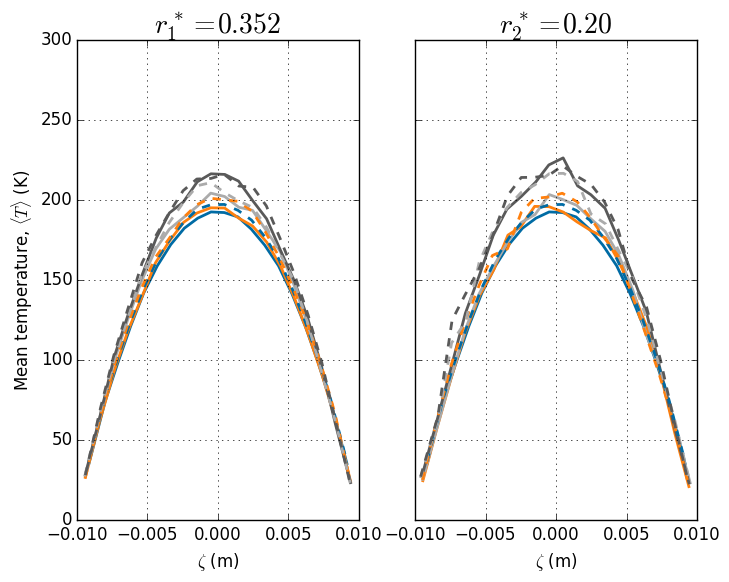
\includegraphics[width=\textwidth]{figures/64-percent-T-profiles.png}
%                \caption{Initial packing fraction of $\phi_2 = 0.64$.}
%                \label{fig:64-T-profile}
%        \end{subfigure}
%        \caption{Solid lines are cases where gravity is in the $\chi$ direction, dashed lines for gravity in the $\zeta$ direction; color is by percent of crushed pebbles, $\eta$.}
% \label{fig:T-profiles}
% \end{figure*}


%---------------------------------------------------------------------------------------
% TABLES
%---------------------------------------------------------------------------------------
\begin{table}[ht]
\centering
\caption{Mechanical and thermal properties of ceramic pebbles in the DEM domain. Aside from $E_s$, properties come from \cite{Gierszewski1998} with $\epsilon = 0.2$}
\label{tab:peb-props}
\resizebox{0.45\textwidth}{!}{%
\begin{tabular}{@{}lcS[table-format=3.2]@{}}
\toprule
%properties are coming from the lit_props.py file in the thesis scripts folder. Double check if you want
Property                                           & Symbol    & \text{Value} \\ \midrule
Young's modulus (\si{\giga\pascal})                & $E_s$     & 60.    \\
Poisson ratio                                      & $\nu_s$     & 0.24  \\
thermal conductivity (\si{\watt\per\meter\per\kelvin}) & $k_s$     & 1.79   \\
diameter (\si{\meter})                             & $d_p$     & 0.001     \\
pebble-pebble friction coefficient                 & $\mu_s$   & 0.2   \\
pebble-wall friction coefficient                   & $\mu_w$   & 0.2   \\ 
heat capacity (\si{\joule\per\kilo\gram\per\kelvin})   & $c_{s}$     & \num{1.45e3}  \\
thermal expansion coefficient (\si{\per\kelvin})   & $\beta_s$ & \num{1.77e-5}      \\
density (\si{\kilo\gram\per\cubic\meter})          & $\rho_s$  & \num{3.44e3}  \\ \bottomrule
\end{tabular}}
\end{table}

\begin{table}[ht]
\centering
\caption{Mechanical and thermal properties and boundary conditions of structural container in the DEM domain \cite{Fokkens2003}.}
\label{tab:wall-props}
\resizebox{0.45\textwidth}{!}{%
\begin{tabular}{@{}lcS[table-format=3.2]@{}}
\toprule
Property                                           & Symbol    & \text{Value} \\ \midrule
Young's modulus (\si{\giga\pascal})                & $E_w$     & 175.    \\
Poisson ratio                                      & $\nu_w$     & 0.30  \\
thermal conductivity (\si{\watt\per\meter\per\kelvin}) & $k_w$     & 29.0   \\ 
wall temperature (\si{\kelvin})                     & $T_{w,s}$        & 573    \\ \bottomrule
\end{tabular}}
\end{table}

\begin{table}[ht]
\centering
\caption{Transport properties of helium and boundary conditions in the CFD domain; mean values over the temperature range \SIrange{400}{900}{\celsius}.}
\label{tab:fluid-props}
\resizebox{0.45\textwidth}{!}{%
\begin{tabular}{@{}lcl@{}}
\toprule
% properties in excel sheet in thesis scripts folder
Property                                           & Symbol    & \text{Value} \\ \midrule
thermal conductivity (\si{\watt\per\meter\per\kelvin}) & $k_f$     & \num{3.40e-1}   \\
heat capacity (\si{\joule\per\kilo\gram\per\kelvin})   & $c_{f}$     & \num{5.19e3}  \\
density (\si{\kilo\gram\per\cubic\meter})          & $\rho_f$  & \num{5.38e-2}  \\
kinematic viscosity (\si{\meter\per\second\squared})   & $\lambda_f$ & \num{8.52e-4}      \\ 
thermal diffusivity (\si{\meter\per\second\squared})   & $\alpha_f$ & \num{1.28e-3}      \\ 
wall temperature (\si{\kelvin})                     & $T_{w,f}$        & 573    \\ 
inlet temperature (\si{\kelvin})                    & $T_i$            & 573    \\ \bottomrule
\end{tabular}}
\end{table}



\subsubsection{Modeling crush events}
Models have been proposed in the past which translate experimental measurements of granular crushing into contact forces in an ensemble to predicty granular crushing, \textit{e.g.} Refs.~\cite{Gan:2010kc,Russell2009,Zhao2012,VanLew2015a,Annabattula2014}, but no validation has set any model apart as yet. Here, packed beds experience artificial pebble-crushing events for which a chosen percentage, $\eta$, of initial pebbles (at randomized locations) fragment. Four crush percentages are used: $\eta = 0, 1, 3, 5\%$. Numerical models of crush events themselves have received attention. Annabattula, Zhao, and Gan attempted to model a crushing event as either a reduction in radius of the crushed pebble or a reduction in Young's modulus \cite{Annabattula2011,Zhao2013,Annabattula2012a}. Van Lew \textit{et al}~made similar simplifications when they considered a crushed pebble as being removed from the force network, thus being removed from the DEM domain \cite{VanLew2014}. 

%None of the approaches discussed above have been fully validated due to a lack of experimental results. 
Building upon the theories of earlier models, we replace a parent pebble of radius $r$ with $N_c$ smaller daughter fragments, each of equal radius, $r_c$. After a crushing event, fragments are free to resettle through interstitial gaps in the pebble bed and original pebbles respond in kind with re-arrangement into a new metastable packing structure.  To conserve volume between pre- and post-crush, we can relate the number of daughter fragments to the radius ratio between fragments and parent, $r^* = r_c/r$, as $N_c = (1/r^*)^{3}$. Experimental studies of crushing brittle pebbles show many different modes of fragmentation, often with highly irregular sizes (see \textit{e.g.} Ref.\cite{Wu2004}). As a first effort, we compare the effect of fragmentation size by studying two different values, $r^*_1 = 0.52$ and $r^*_2 = 0.2$ which results in $N_{c,1} = 23$ and $N_{c,2} = 125$ daughters per crushed parent (at $\eta = 5\%$, for $r_2^*$ the system expands to \num{43200} pebbles). Conservation of energy of crush event is enforced by setting the temperature of daughter fragments to the parent pebble at the moment of crushing. After insertion, the daughter fragment temperatures then evolve in time with standard integration.







\subsection{Results \& Discussion}
In \Cref{fig:inset}, a bed of 64\% initial packing with 5\% of pebbles broken into fragments of size $r_2^* = 0.2$ is shown; vectors of flow field, colored by fluid temperature, are seen moving through the bed. The inset image qualitatively demonstrates how the fluid field aids in equilibrating temperatures of fragments with neighboring larger pebbles in spite of light physical contact between pebbles. 

\begin{figure}[!h]
    \centering
    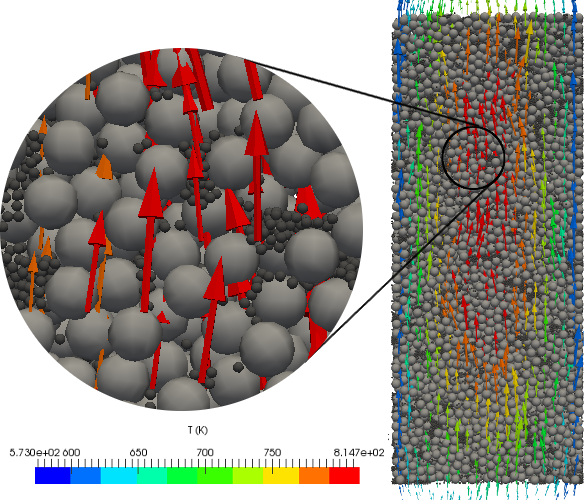
\includegraphics[width = 0.75\textwidth]{figures/pebble_inset_2.png}
    \caption{Showing the case for $\phi_2 = 0.64$, $\eta = 5\%$ with fluid velocity vectors colored by temperature. Inset image reveals size discrepancies between fragments and pebbles and the ensemble interaction with fluid flow.}\label{fig:inset}
\end{figure}

Several cross-sections are created at mid-planes in $z$. Representative results are taken from 64\% packings of $\zeta$- and $\chi$-configurations and compared against their respective $\eta = 5\%$, $r_2^*$ conditions, shown in \Cref{fig:1,fig:3}. The numbered zones of the beds will be discussed shortly.

\begin{figure}[!ht]
    \centering
    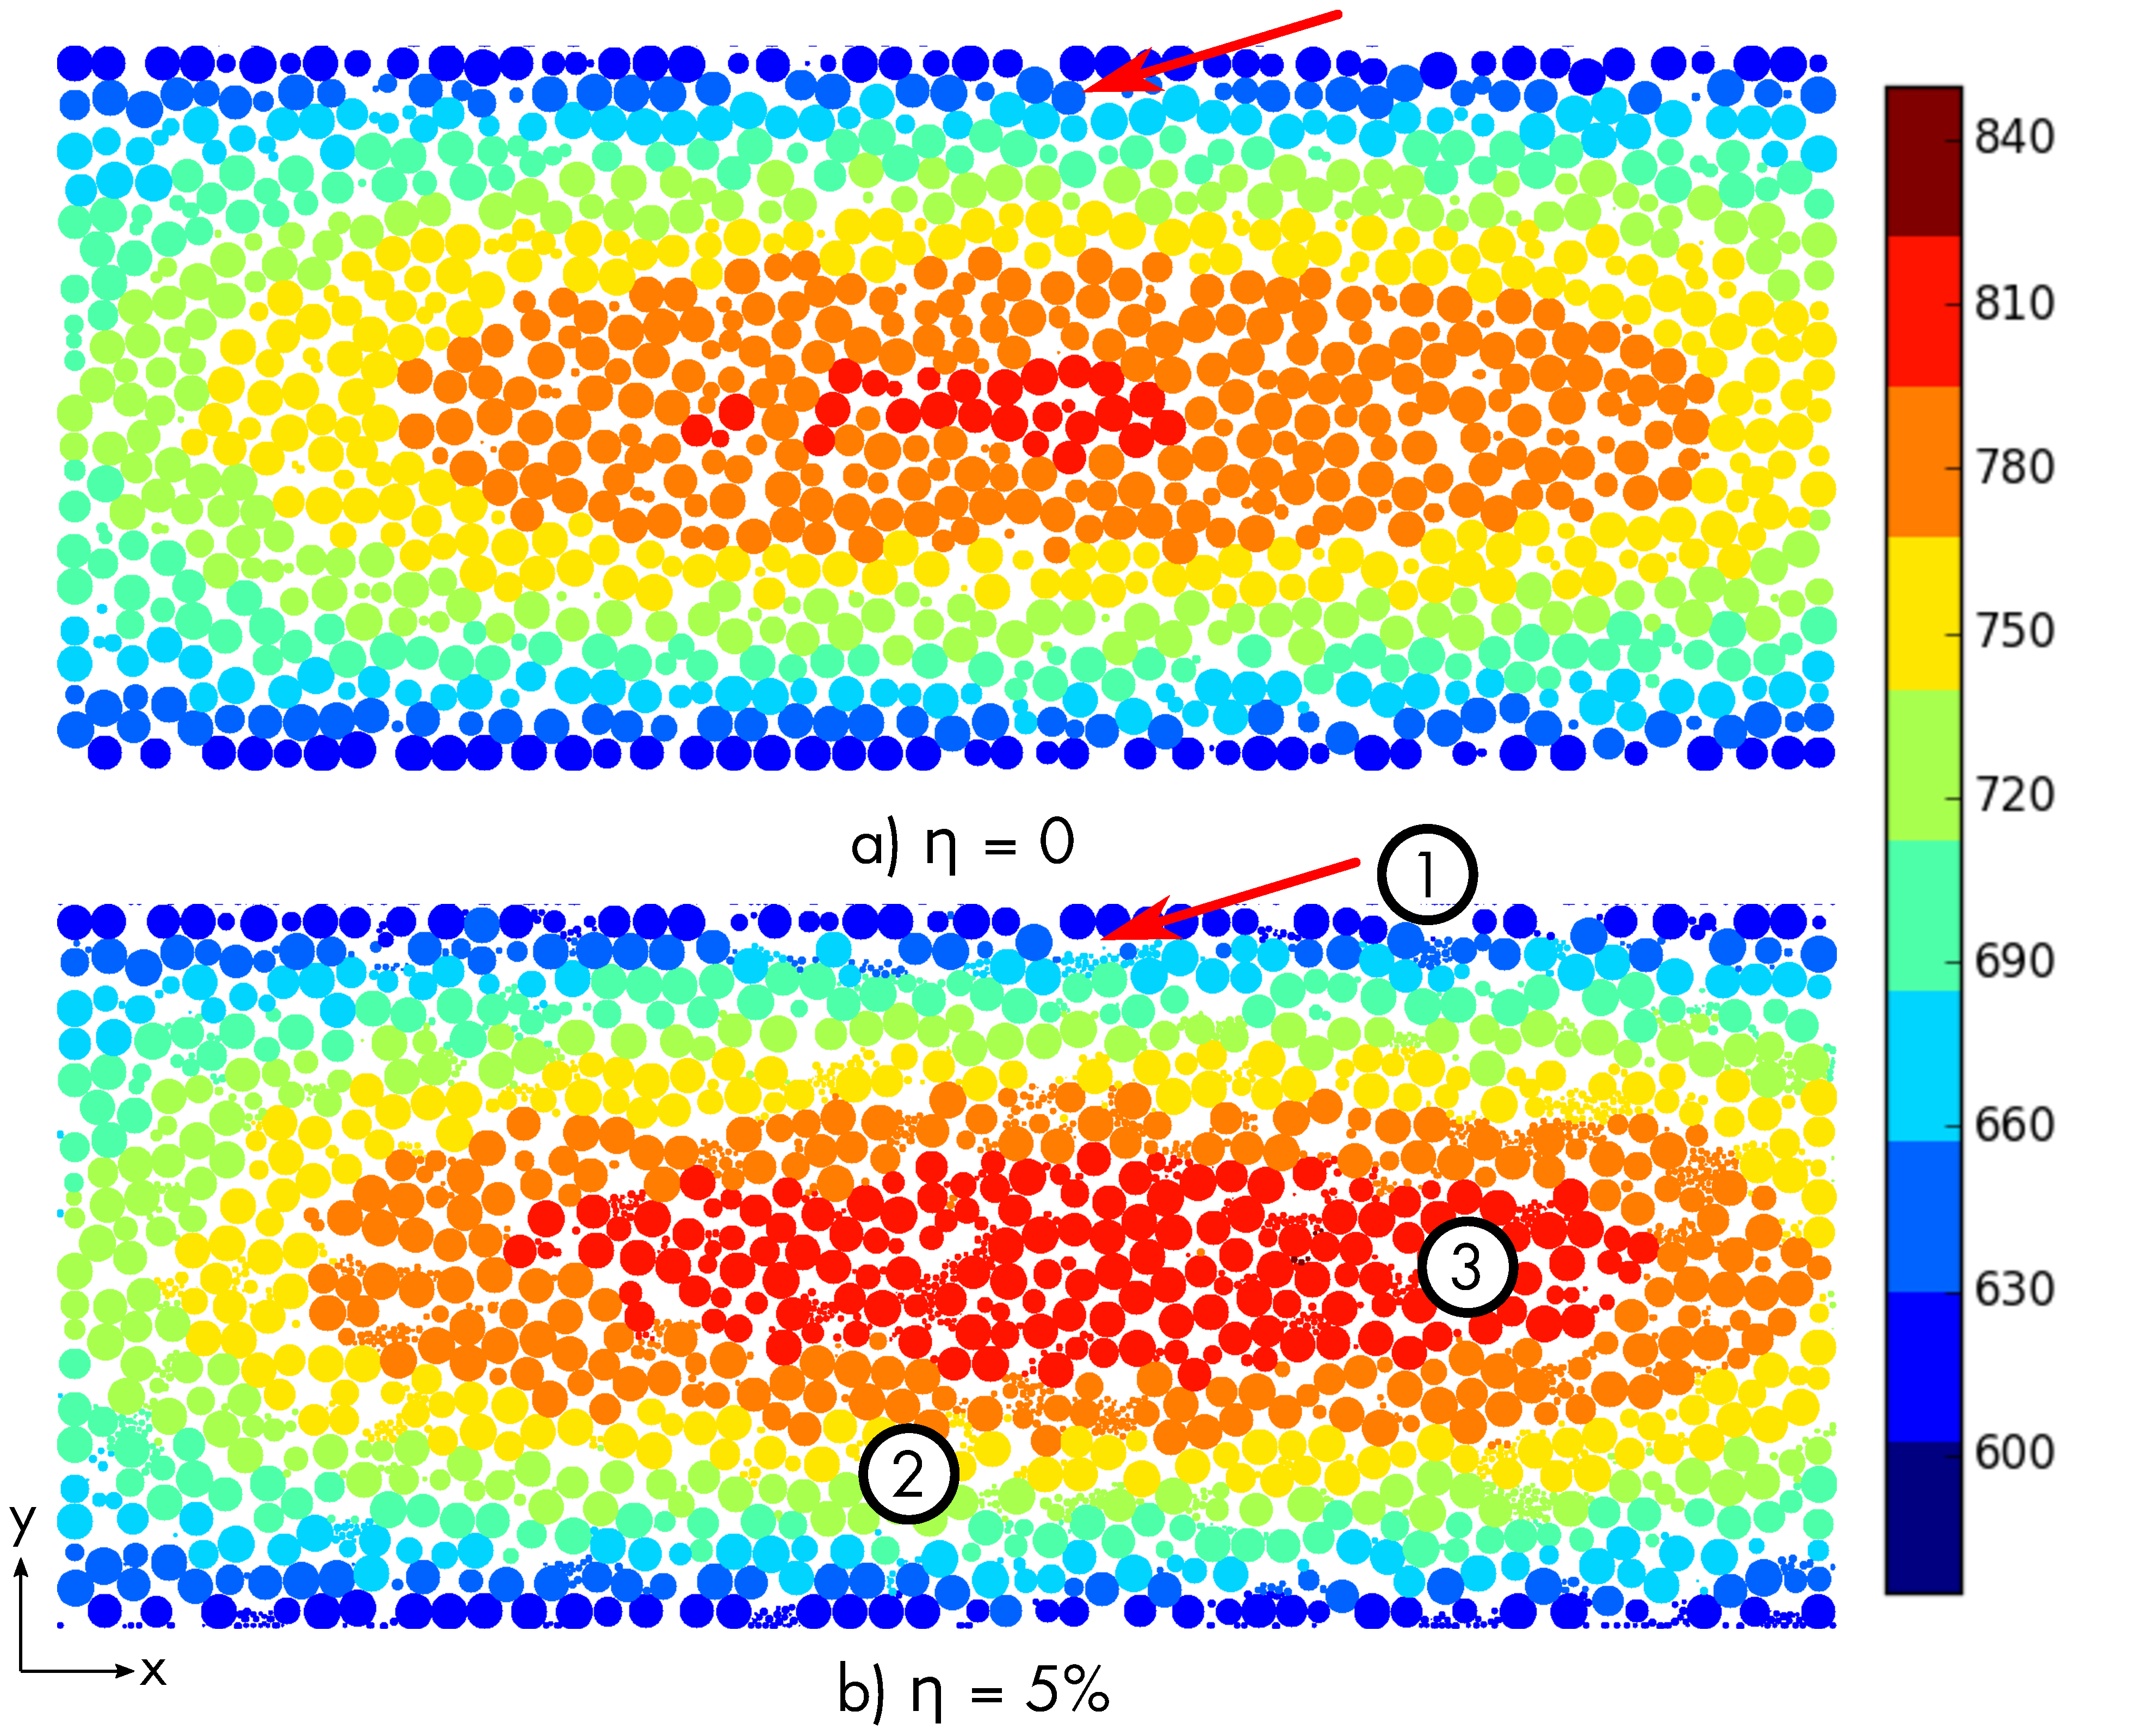
\includegraphics[width = \textwidth]{figures/z-64-discrete.eps}
    \caption{Cuts at the mid-plane of $z$ for $\zeta$-config beds. (a) bed initially packed to $\phi_2$, and (b) bed with crushing of $\eta_5$ pebbles with particle size $r_2^*$. Three important zones have been identified}\label{fig:1}
\end{figure}

\begin{figure}[!ht]
    \centering
    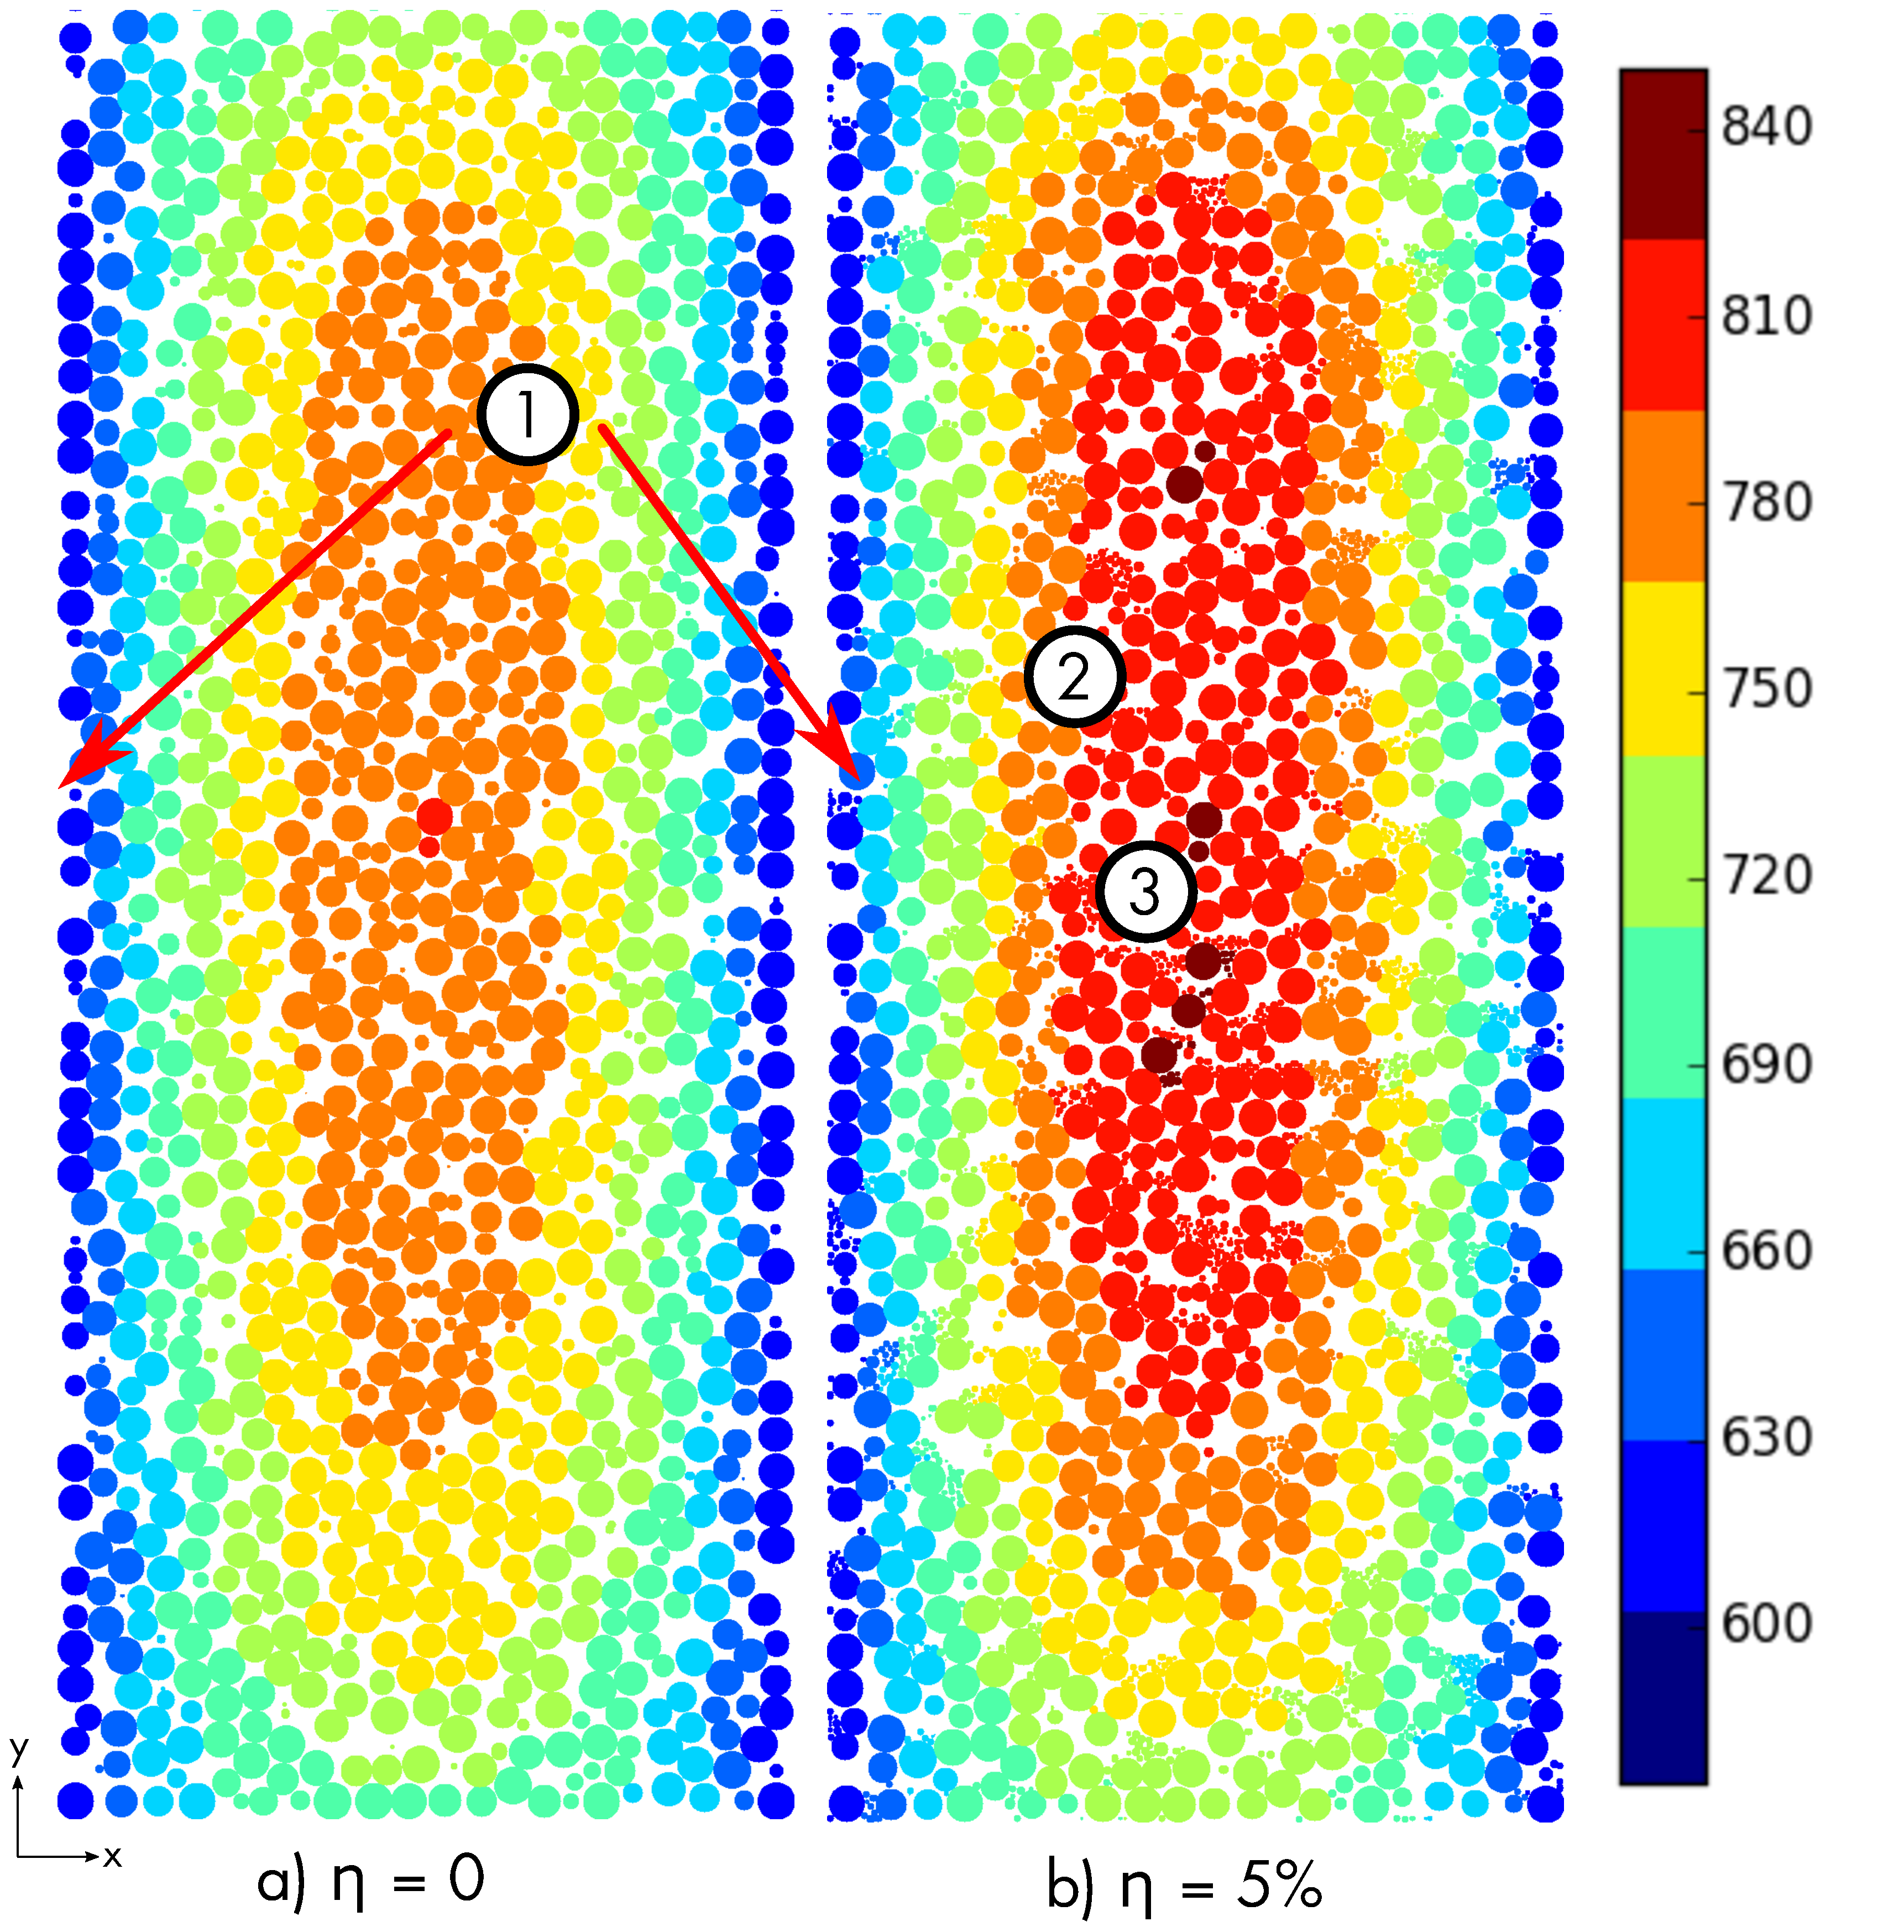
\includegraphics[width = 0.75\textwidth]{figures/x-64-discrete.eps}
    \caption{Cuts at the mid-plane of $z$ for $\chi$-config beds. (a) bed initially packed to $\phi_2$, and (b) bed with crushing of $\eta_5$ pebbles with particle size $r_2^*$. Three important zones have been identified}\label{fig:3}
\end{figure}

Mean reduced temperatures in beds are found in slices of width $\Delta\zeta$ along $\zeta$. Pebble-weighted mean values are found as $\langle T\rangle = \frac{1}{V_n}\sum_{j}^n (T_j-T_w) V_j$, for $n$ pebbles of temperature $T_j$ consuming a total volume $V_n$ in the slice. Demonstrative cases of $\phi_2 = 0.64$ with $r_2^* = 0.2$ are given in \Cref{fig:64-T-profile} as functions of granular crushing percentage.

Pebble bed internal stresses are found from normal and tangential forces that make up force networks in ensembles. Following the formulations described by Gan \& Kamlah \cite{Gan:2010uq}, the magnitude of the stress tensor, $|\sigma|$, is found for every pebble bed at steady-state heating and then normalized against initial ($\eta=0$) beds for respective configurations, given in \Cref{fig:eta-sigma}.%considered configuration, $\sigma^*=|\sigma|_\eta/|\sigma|_{\eta_0}$. %Normalized bed stresses decrease with increasing granular fragmentation, as seen in \Cref{fig:eta-sigma}, for all initial packings and bed orientations, by about 30 to 60\%.

A total mean bed temperature is found from all pebbles in the system as $\langle T\rangle_{tot} = \frac{1}{V_N}\sum_{j}^N (T_j-T_w) V_j$ where $N$ is the total number of ensemble pebbles. The total mean bed temperature is also normalized against initial packing cases of each respective set of beds. Results for all beds are given in \Cref{fig:eta-theta}. Maximum temperature rises of every bed are also found, $T_m = \max(T) - T_w$, and normalized against the maximum temperature in the initial packing of each respective set of beds. To avoid aberrent results from a bed which might have a single, very high temperature pebble, the maximum temperature, $\max(T)$, is calculated as a mean value of the 50 highest temperature pebbles. The results are given in \Cref{fig:eta-T_max}. In addition to total mean bed temperature, maximum temperature rise is also an important factor in evaluation of a pebble bed.

Lastly, we consider how far pebble fragments travel in the bed after a crushing event. Total displacements from the moment of crush event to final resting, $|\Delta h|$, are normalized against the original pebble diameter, $|\Delta h|/d_p$. Histograms for 64\% packing fractions of $\chi$- and $\zeta$-configurations at 5\% pebble crushing are given in \Cref{fig:displacement_hists}. These two beds saw the most settling, all other beds tested saw considerably less fragment displacements.





% \begin{figure}[!h]
% \centering
% 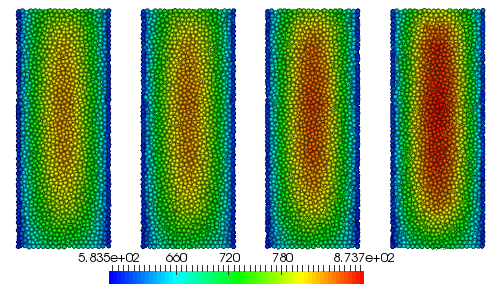
\includegraphics[width = 0.4\textwidth]{figures/62x-edit.png}
% \caption{Pebble temperature distributions in the $\chi$-config with $\phi_1 = 0.62$ initial packing increase with increased granular damage, from left to right is $\eta = 0, 0.01, 0.03, 0.05$.}\label{fig:62xpebs}
% \end{figure}

% numeric integration of mean temperature profiles, $\Theta = \frac{1}{L}\int\langle T \rangle \,\mathrm{d}\zeta$, where $L$ is the \SI{20}{\milli\meter} width of $\zeta$; $\Theta$ is plotted in \Cref{fig:eta-theta}.



% \begin{figure*}[!ht]
%        \centering
%        \begin{subfigure}[b]{0.45\textwidth}
%                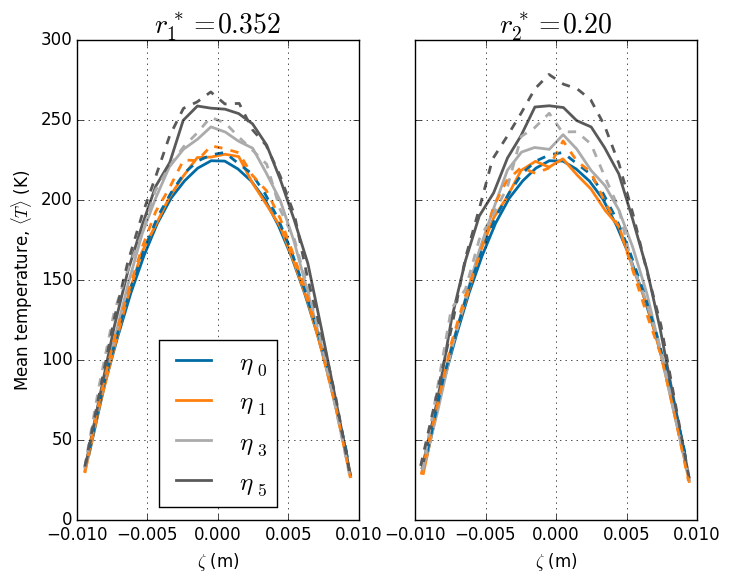
\includegraphics[width=\textwidth]{figures/62-percent-T-profiles.png}
%                \caption{Initial packing fraction of $\phi_1 = 0.62$.}
%                \label{fig:62-T-profile}
%        \end{subfigure}%
%        ~ %add desired spacing between images, e. g. ~, \quad, \qquad, \hfill etc.
%          %(or a blank line to force the subfigure onto a new line)
%        \begin{subfigure}[b]{0.45\textwidth}
%                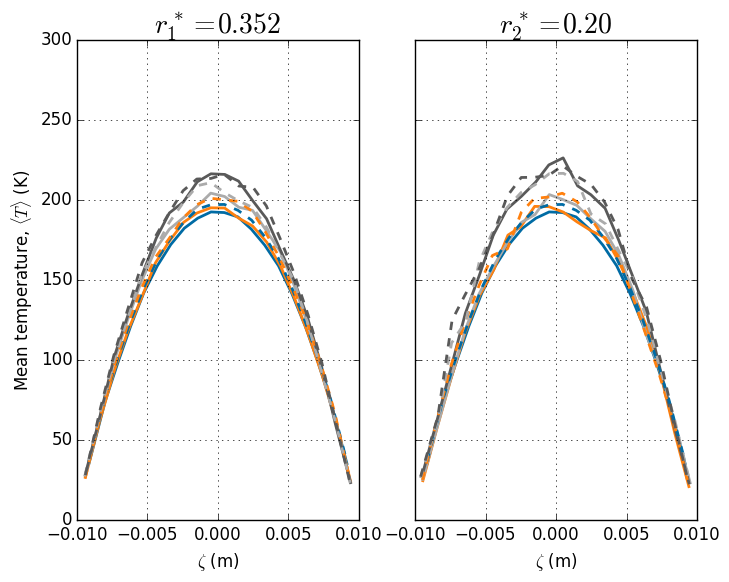
\includegraphics[width=\textwidth]{figures/64-percent-T-profiles.png}
%                \caption{Initial packing fraction of $\phi_2 = 0.64$.}
%                \label{fig:64-T-profile}
%        \end{subfigure}
%        \caption{Solid lines are cases where gravity is in the $\chi$ direction, dashed lines for gravity in the $\zeta$ direction; color is by percent of crushed pebbles, $\eta$.}
% \label{fig:T-profiles}
% \end{figure*}

%

% \begin{figure*}[!ht]
%        \centering
%        \begin{subfigure}[b]{0.45\textwidth}
%                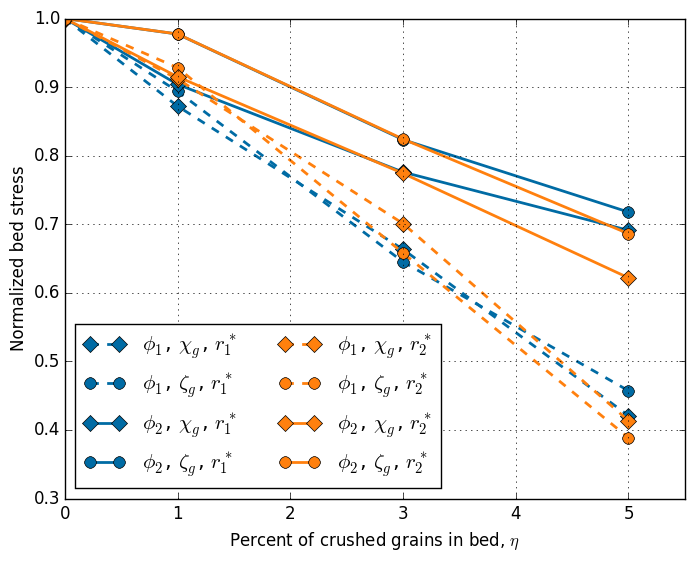
\includegraphics[width = \textwidth]{figures/eta-sigma.png}
%               \caption{Lower packing fractions have lower initial bed stress, stress decreases with increased granular crushing. }\label{fig:eta-sigma}
%        \end{subfigure}%
%        ~ %add desired spacing between images, e. g. ~, \quad, \qquad, \hfill etc.
%          %(or a blank line to force the subfigure onto a new line)
%        \begin{subfigure}[b]{0.45\textwidth}
%                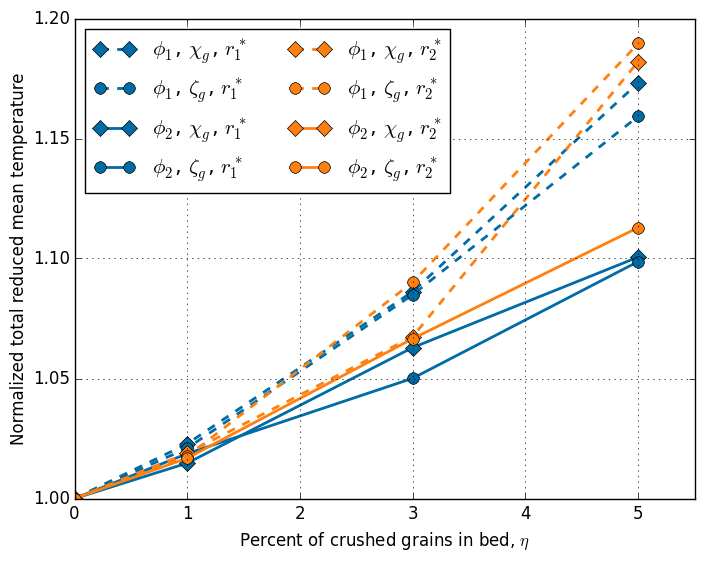
\includegraphics[width = \textwidth]{figures/eta-theta.png}
%               \caption{Lower packing fractions have higher initial bed temperatures, mean temperatures increase with increased granular crushing.}\label{fig:eta-theta}
%        \end{subfigure}
%        \caption{Changes in temperature and bed stress as functions of granular damage percent, $\eta$, with varying parameters of packing fraction, $\phi_1 = 0.62$, $\phi_2 = 0.64$; fragmentation radius ratio, $r_1^* = 0.52$, $r_2^* = 0.2$; and configuration, $\chi_g$ is $\chi$-config, $\zeta_g$ is $\zeta$-config.}
% \label{fig:eta-plots}
% \end{figure*}
\begin{figure}[!t]
    \centering
    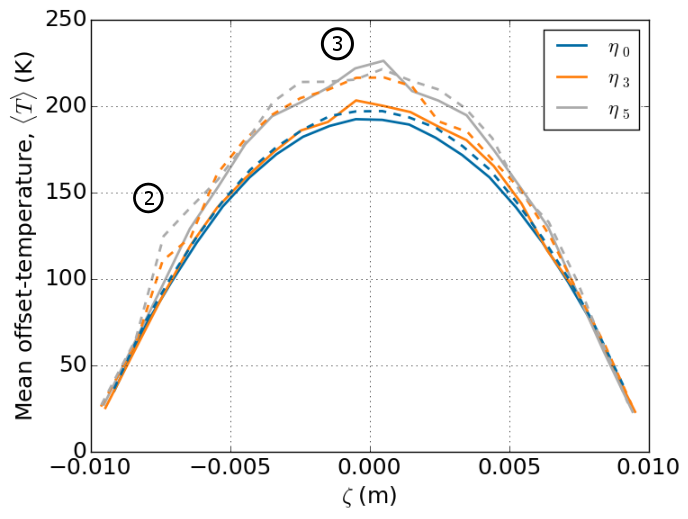
\includegraphics[width=0.5\textwidth]{figures/64-percent-T-profiles-reduced.png}
    \caption{Mean temperature profiles, $\langle T \rangle$, along $\zeta$ in beds with initial packing fractions $\phi_2 = 0.64$, fragmentation sizes were $r_2^*$. Solid lines are $\chi$ configurations, dashes lines are $\zeta$ configurations. Fragmentation settling of $\zeta$-configs are seen in `lumps' near Zone (2) and in the $\chi$-config spike in zone (3).}
    \label{fig:64-T-profile}
\end{figure}

\begin{figure}[!t]
    \centering
    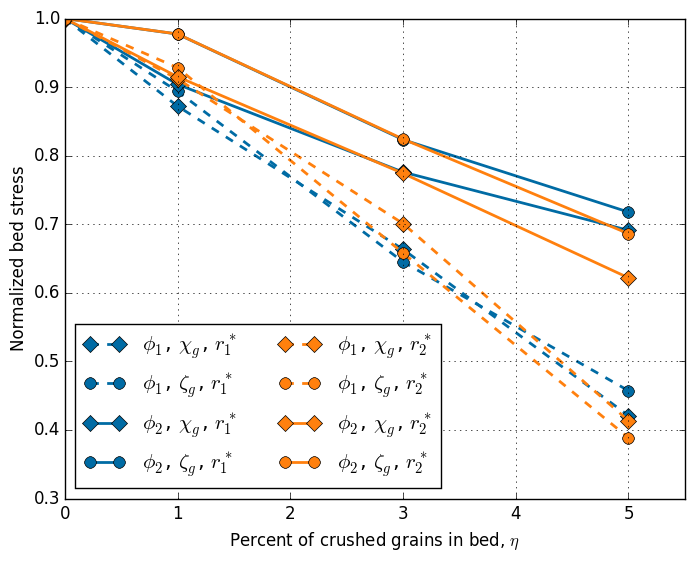
\includegraphics[width = 0.5\textwidth]{figures/eta-sigma.png}
    \caption{Dashed lines represent the lower packing fraction, $\phi_1 = 0.62$, solid lines are $\phi_2 = 0.64$. Markers are: $\circ$ for $\zeta$-config, $\diamondsuit$ for $\chi$-config. Color differentiates the fragment radius ratio. Contact force relaxation is more rapid for lower packing fractions.}\label{fig:eta-sigma}
\end{figure}

\begin{figure}[!t]
    \centering
    \includegraphics[width = 0.5\textwidth]{figures/eta-theta.png}
    \caption{Dashed lines represent the lower packing fraction, $\phi_1 = 0.62$, solid lines are $\phi_2 = 0.64$. Markers are: $\circ$ for $\zeta$-config, $\diamondsuit$ for $\chi$-config. Color differentiates the fragment radius ratio. Lower packing fraction is the most dominant parameter for overall bed temperature. Amongst the same packing fraction, fragment size is most influential factor.}\label{fig:eta-theta}
\end{figure}

\begin{figure}[!t]
    \centering
    \includegraphics[width = 0.5\textwidth]{figures/eta-T_max.png}
    \caption{Dashed lines represent the lower packing fraction, $\phi_1 = 0.62$, solid lines are $\phi_2 = 0.64$. Markers are: $\circ$ for $\zeta$-config, $\diamondsuit$ for $\chi$-config. Color differentiates the fragment radius ratio. The dominant parameter influencing maximum bed temperature varies as a function of the number of crushed pebbles in the bed.}\label{fig:eta-T_max}
\end{figure}

\begin{figure}[!t]
    \centering
    \includegraphics[width = 0.65\textwidth]{figures/displacement_histograms.png}
    \caption{Normalized displacement histograms. $\chi$-config: 59.7\% of fragments travel up to \SI{1}{\milli\meter} and 8.2\% travel more than \SI{2}{\milli\meter}; $\zeta$-config: 60.7\% of fragments travel up to \SI{1}{\milli\meter}, 7.9\% travel more than \SI{2}{\milli\meter}.}\label{fig:displacement_hists}
\end{figure}

% Conductive heat transport in granular materials is dependent on normal forces between pebbles, and normal forces need not be isotropically distributed through beds. To investigate directional dependence, we calculate angular distributions of granular contacts and forces between every pair of interacting pebbles in the ensemble. Contact angle is measured between vectors pointing between contacting pebbles and $\zeta$. In other words, the most direct path for heat out of the system is along contacts at angles of $\theta=0,\pi$; magnitudes of contact forces around those angles dictate the ability of systems to discharge heat to coolant. A mean contact force, $\langle F_n \rangle$, is found inside wedges of $\Delta\theta$ in the same manner described above for ensemble-averaged temperature values. Mean forces for varying fragmentation amount, fragmentation size, initial packing density, and orientation are plotted in \Cref{fig:force-polars}.
% , the stress tensor, $\mathbf{\sigma}$, is
% \begin{equation}
%   \sigma_{jk} = \frac{1}{V}\left(\sum_c d_0 f^{(n)} n_jn_k + \sum_c d_0 f^{(t)} n_jt_k\right)
% \end{equation}
% where $c$ indicates a contact pair of pebbles, $d_0$ is the separation distance between the centroids of the pebbles, $f^{(n)}$ and $f^{(t)}$ are the projected normal and tangential components of the contact force between the pair, and $\mathbf{n}$ and $\mathbf{t}$ are the normal and tangential unit vectors.
% \begin{figure*}[!tp]
%        \centering
%        \begin{subfigure}[b]{0.45\textwidth}
%                \includegraphics[width=\textwidth]{figures/62-percent-polar-forces.png}
%                \caption{Initial packing fraction of $\phi_1 = 0.62$.}
%                \label{fig:62-force-polar}
%        \end{subfigure}%
%        ~ %add desired spacing between images, e. g. ~, \quad, \qquad, \hfill etc.
%          %(or a blank line to force the subfigure onto a new line)
%        \begin{subfigure}[b]{0.45\textwidth}
%                \includegraphics[width=\textwidth]{figures/64-percent-polar-forces.png}
%                \caption{Initial packing fraction of $\phi_2 = 0.64$.}
%                \label{fig:64-force-polar}
%        \end{subfigure}
%        \caption{Ensemble-average contact forces in wedges of angle $\Delta\theta$: solid lines are cases where gravity is in the $\chi$ direction ($\chi$-config), dashed lines for gravity in the $\zeta$ direction ($\zeta$-config); color is by percent of crushed pebbles.} %Grain orientation is such that polar angles of $\theta = 0,\pi$, are the directions of heat transfer in the bed.}
% \label{fig:force-polars}
% \end{figure*}

Analyzing results of all the pebble beds in this study revealed two main contributors to bed temperatures with resettling from pebble crushing: final settling location of fragment particles and overall contact force relaxation. The two interacting contributors were found to be expressed to different extents depending on crush amount and bed configuration.

Bed stress (a global measure of inter-particle contact forces) is predominately a function of initial packing fraction alone, as seen in \Cref{fig:eta-sigma}. Smaller initial packing fractions had their internal stress reduced more rapidly as pebbles crushed in the ensemble. Breeder orientation appears to have less impact on stress relief than size of crush fragments. Due to the inter-connected nature of the force network, and geometry of beds studied here, resettling in beds and contact force relaxation is uniform throughout the beds. Thus we expect reductions in contact forces to directly result in an overall increase of bed temperatures. This is reflected in the curves of \Cref{fig:eta-theta}. Total mean temperatures of $\phi_1 = 0.62$ beds increased between \numrange{16}{19}\% at $\eta = 5\%$. Yet beds initially packed to $\phi_2 = 0.64$ increased by only \numrange{10}{13}\% at the same value of crushed pebble amount.

Fragment settling location, on the contrary, is strongly dependent on fragment size and breeder orientation. The pebble fragments have very poor thermal conductance to neighboring pebbles because they do not exist in the larger pebbles' force network. Fragment temperatures are therefore mostly regulated by convection with interstitial helium and their influence on bed temperatures is much more complex. The effect becomes more pronounced with decreasing size of fragments.

To identify the effects of fragment settling, we look to \Cref{fig:displacement_hists} and the several zones demarcated in the results of \Cref{fig:1,fig:3}. The displacement histogram reveals settling as a relatively localized event. Most fragments, even in this case of smallest fragment size and largest crushing amount, remain approximately at the location of the parent pebble; for both configurations, approximately 60\% travel less than 1 pebble diameter (\SI{1}{\milli\meter}). However, in both configurations, approximately 8\% of fragments travel more than 2 diameters, and those pebbles have a significant impact on the ensembles overall thermal response.

In $\zeta$-configuration beds, pebbles traveling more than a few pebble diameters will move between colored isotherms drawn in \Cref{fig:1}. For example we can see the fragment group identified in Zone (1) as moving downward, away from the top wall. Similarly, when pebbles in Zone (3) are crushed, some of the fragments tumble downward into Zone (2) before coming to rest where they continue to receive volumetric heating. Thus the fragments, with poor thermal conductance, increase heating in the regions where they settle. The effect is seen in the $\eta = 3, 5\%$ temperature profiles in \Cref{fig:64-T-profile} that are asymmetric with lower temperatures in the top half (above Zone (3)) and higher temperatures in the region near Zone (2).

In contrast, $\chi$-config beds respond much differently to pebble fragment settling. We again see from cross-sections in \Cref{fig:3} a pebble identified in Zone (1) that breaks but remains in that zone after settling. The trend continues in other regions of the bed. Because of the gravity's effect, when pebbles are crushed in the $\chi$-config beds, they fall downward but remain generally in the same isotherm, as drawn in \Cref{fig:3}. According to \Cref{fig:64-T-profile}, the effect of pebble crushing has little effect up to 3\% of damaged pebbles. But suddenly at $\eta = 5\%$, the combination of reduced overall bed stress and fragmentation heating causes the maximum bed temperature to jump above all other $\phi = 64\%$ beds (see \Cref{fig:64-T-profile} and \Cref{fig:eta-T_max}). The temperature increase in this $\chi$-config bed is due to the accumulation of pebble fragments that remain in Zone (3), only tumbling to lower heights. Helium that enters the $\chi$-configuration bed reaches higher temperatures more quickly due to the increased heating from fragments which settled at lower heights of $y$. Helium then continues to heat from the many fragments in Zone (3) which ultimately results in the highest maximum bed temperatures (for the given packing fraction). This can also be seen with comparison between \Cref{fig:1,fig:3}: the $\chi$-config bed reaches the $780$~\si{\kelvin} contour at a much lower height than the $\zeta$-configuration. 

%in each configuration is the near-wall region where pebbles contact walls. In $\chi$-config bed in \Cref{fig:3}, we can see how pebble fragments tumble downward but generally remain in the near-wall region of Zone (1). Conversely, we see clearly in the $\zeta$-config bed of \Cref{fig:1} that some fragment groups leave the region and resettle downward toward the bed's central region. The differences in settling between the two configurations is consistent when we consider pebble behavior in other zones.

%Zones (2) are the moderate temperature regions of \Cref{fig:1,fig:3}, the approximate location is also shown on temperature profiles in \Cref{fig:64-T-profile}. For $\zeta$-configs, temperatures shown in \Cref{fig:64-T-profile} demonstrate an asymmetric lump in profile that is absent in $\chi$-config beds. Increases in Zone (2) temperatures for $\zeta$-config beds are due to the fraction of pebbles which freely tumble through interstitial gaps, influenced by gravity, into Zone (2) from other regions. Once settled, the increased masses of ceramic in Zone (2) then create additional heating from the volumetric source. It should be noted that the exact location of the `lumps' in temperature profiles measured here are unique to the pebble bed considered in this study and the random location at which the fragments accumulated, however the phenomena of increased temperature in the lower-half of $y$-locations of beds with crushed pebbles will consistently appear. As for the $\chi$-configurations, pebbles broken in Zone (2) see their daughter fragments remain in Zone (2) as they tumble in the $y$-direction, regardless of the distance. No added mass in the region results in no abnormal increases in Zone (2) temperature profiles; only overall increases of temperatures are witnessed. 

%For $\zeta$-config beds, a similar effect of fragment-travel into and out of Zone (3) occurs, long-distance traveling of the roughly 10\% of pebbles in $\zeta$ configuration contributes to spreading heat generation from the high temperature regions into regions at lower heights of $y$. However, in $\chi$-config beds, pebbles that crush in Zone (3) again have fragments which generally remain in Zone (3) regardless of distance traveled. The accumulating pebble fragments in Zone (3) continue to receive nuclear heating but have very poor contact conductance with neighboring pebbles. The flowing helium purge gas prevents runaway high temperatures of these fragments but the end results are higher maximum temperatures. In the case of $r_2^*$ at $\eta = 5\%$, we see in \Cref{fig:eta-T_max} the maximum temperatures in $\chi$-config beds overtake the maximum temperatures of similar $\zeta$-config beds. This large increase in maximum temperature rise is due entirely to small fragments accumulation in Zone (3), the similar bed of $\zeta$-configuration shows a much lower maximum bed temperature rise. It is also interesting to note the two beds with smallest temperature rise among any studied here were $\zeta$-configurations. Yet at the same time, those two beds saw similar or more increase in overall bed temperatures in comparison to $\chi$-configurations. These results demonstrate the effect of pebble fragments traveling between zones in $\zeta$-config beds: increasing temperatures in moderate-temperature zones with a trade-off of decreased temperatures in high-temperature zones.

%Looking to \Cref{fig:eta-T_max}, among all the solid lines ($\phi_2 = 0.64$) we see a large jump in bed temperature rise only for the $\chi$-config bed at $\eta = 5\%$ with $r_2^*$; the maximum bed temperature even jumps above most of the less-tightly packed $\phi_1$ beds. It is interesting to note that a similar set of parameters ($\phi_2, r_2^*, \eta_5$) in the $\zeta$-configuration shows a much lower maximum bed temperature rise. Furthermore, 

%, the phenomena of inter-granular resettling strongly impacting temperature rises only occurred for beds with small fragmentation sizes, $r_2^* = 0.2$; see $(\phi_2, \chi_g, r_w^*)$ at $\eta = 5\%$. This is attributed to the tightly packed structures of these well-packed beds. But when the initial packing fraction was reduced, $\phi_1$, for instance, increases in maximum temperatures due to fragment resettling was seen even for larger fragments, $r_1^* =  0.52$. 

%Results shown here illustrate many unique features of heat transfer in granular materials with crushed pebbles and fluid flow. 
%From the temperature profiles of \Cref{fig:T-profiles}, smooth parabolic temperature profiles for initially-packed beds ($\eta = 0$ for both $\phi_{1,2}$) indicate constant $\keff$ values and support the use of continuum theory for those granular assemblies. However, for $\eta > 0$, at all packing fractions and fragmentation radius ratios, temperature profiles become increasingly jagged with large jumps in mean temperatures along $\zeta$ due to heating of crush fragments and distribution of contact forces. Standard models with continuum treatment of granular material cannot predict this manner of inhomogeneous transport of heat in pebble beds. The $\keff$ model must be re-evaluated for use with crushable granular materials.

%for larger crush fragments ($r_1^*$), temperature profiles remained near-perfect parabolas, indicating constant $\keff$ and rough applicability of continuum, for all initial packing fractions and granular crush amounts. However, when fragments were smaller ($r_2^*$), the profiles became more jagged deviation began to occur as crush amount increased. The importance of the profile is in its indication of a constant $\keff$ through the granular material; from the boundary conditions of the system, the more constant the $\keff$, the more perfectly parabolic the temperature profile. This has important repercussions on the the $\keff$ treatment of the granular ceramic as a continuum medium in macro-scale simulations. 

%In \Cref{fig:eta-theta}, total mean temperatures as functions of granular crushing amount are given. Some observable trends: 1) lower initial packing fractions, \textit{i.e.} $\phi_1$, see greater reductions in bed stress and greater mean bed temperatures as pebbles are crushed ; 2) beds with with heat outflow in the direction of gravity ($\zeta$-config) generally had higher bed temperatures for all granular crushing amounts compared to beds with heat outflow perpendicular to gravity ($\chi$-config); 3) size of granular fragment had little impact on bed stresses (until $\eta = 5\%$), but generally beds with smaller fragments had higher temperatures due to small fragments having very small conductive heat transport; 4) when considering fragmentation, there is a weak relationship of internal stress to mean bed temperature. For example, comparing cases of $\phi_2$, $\chi_g$ with the two $r^*_{1,2}$ as functions of $\eta$. For $\eta = 0, 1, 3\%$, stress falls to almost identical values (\Cref{fig:eta-sigma}), yet temperatures for the bed with $r_2^*$ have much higher mean temperatures for all fragmentation amounts.
%If one were to rely only on indirect measurements of pebble bed integrity, \textit{i.e.} measurements of bed pressure load, changes to pebble bed temperature might go unnoticed.

%The polar angle, $\theta$, shown from $0$ to $\pi$ in \Cref{fig:force-polars} is always measured as the angle from $\zeta$ direction -- the mean direction for heat transport to coolant. Thus for all cases, the angles near $\theta = 0,\pi$ correspond to pebbles contacting and transferring heat towards the coolant. Whereas contact between pebbles at angles near $\theta = \pi/2$ correspond to contacts approximately along isotherms in $\chi$ directions (see \Cref{fig:62xpebs}) with little impact on bed heat removal. These plots are more indicative of a pebble bed's ability to transport heat to coolant than bed stresses in \Cref{fig:eta-sigma}. Configurations with $\chi$-direction gravity see higher contact forces near $\theta = 0, \pi$ for all parameters, compared to similar $\zeta$-config beds; likewise the temperatures of $\chi$-config beds are always cooler than similar $\zeta$-config beds. 
%For $\chi$-config cases of \Cref{fig:62-force-polar,fig:64-force-polar}, forces near $\theta = 0,\pi$ are reduced less as individual pebbles are crushed in the ensemble than comparable $\zeta$-config cases. For example, for $\phi_2$, $r^*_1$, mean contact forces near $\theta=0,\pi$ drop by approximately 51\% for $\chi$-configurations whereas mean normal forces drop by nearly 65\% for $\zeta$-configurations. 
%When the internal stress is calculated for pebble beds (for \Cref{fig:eta-sigma}), directional dependence of contact forces is ignored; large forces near $\theta = \pi/2$ mask the reductions in contact forces along heat removal routes. %Therefore overall internal stress of a bed may not drop by a large degree due to large contact forces near $\theta = \pi/2$ directions, but heat transport to boundaries may be strongly affected and temperatures will rise in the bed. 
%This phenomena was observed and mentioned in discussions of \Cref{fig:eta-plots}; and is explainable by directional-dependencies of contact forces and heat transfer in granular systems.


\subsection{Conclusions}
We conducted several multi-scale simulations of granular heat transfer using coupled CFD-DEM simulations of representative tritium-breeding ceramic pebble bed volumes with parametric variations of: bed orientation with respect to gravity, pebble crushing amount, initial packing fraction, and crushed fragmentation size.

There was one general trend observed that reiterates past conclusions from solid breeder research. Namely, more persistent behavior is witnessed in pebble beds with higher initial packing fractions. In this study, the most dominant parameter observed to affect temperatures in pebble beds was the initial packing fraction: beds with higher initial packing fraction had smaller increases in bed temperatures due to pebble crushing. We therefore conclude that manual densification, from either long-term vibration packing or load-induced pre-compaction, must be done to ceramic pebble bed volumes to gain some temperature control during operation in a fusion reactor. To achieve packing fractions of $64\%$ in the relatively small sizes of this study, for example, a load of over \SI{1}{\mega\pascal} was necessary. In the assembly of tritium breeding modules, it must be kept in mind that similar pre-compactions may need to be performed.

As stated earlier, a concern with the $\zeta$ design is the possibility of gap formation between pebble bed and upper walls after bed resettling, particularly after pebble fragmentation. In this study, we found pebble beds initially packed to $\phi = 62\%$ experienced the highest increases in both total average bed temperature as well as maximum temperature rise. The comparably looser packing allowed a quick reduction in bed stresses and consequently a reduction in heat conduction to the upper wall. Nevertheless, no gaps were detected even at 5\% of pebbles crushed. However, temperatures in pebble beds packed to 64\% showed a resistance to fragmentation; overall average temperatures were comparable to $\chi$-configurations, and in fact these EU-style beds had the lowest maximum temperatures for beds with many crushed pebbles. We showed that freedom of fragments to travel between zones in these beds prevented a build-up of loose fragments (and thereby avoided build-up of heating) in the hottest regions.

As for the $\chi$-configurations, we found that when there were not many broken pebbles ($\eta \le 3$\%), these beds generally had lower temperatures in comparison to similar $\zeta$-config beds. But as $\eta$ went above 3\% for many of the beds, the averaged bed temperature and, importantly, the maximum temperature rise actually jumped above the $\zeta$-configurations. We showed that for these beds it was the inability for fragments to move between zones which left many small fragments to settle in the hottest region, further contributing to heating.

From the results we have shown, it is obvious that pebble crushing and bed resettling effects on temperature are complicated, non-linear functions of breeder design and ceramic material employed. We found indications of certain operational spaces for which different designs excelled. For instance, if one were using a material known to have a limited crush strength, one might accept that many pebbles could break (at least up to 5\%, as studied here) over the life of the breeder and choose to employ the $\zeta$-style which avoided large increases in temperature after long operation of the breeder. Alternatively, if one had a ceramic material with a larger crush strength, the $\chi$-design would be preferable as it generally retained lower overall and maximum bed temperatures when fewer pebbles in the ensemble were crushed.

This study was performed on some generic geometries and has provided some generalized conclusions. But in light of the pebble beds' complex responses, as breeder designs continue to evolve into their final form before deployment in ITER, CFD-DEM models should continuously be employed to study the specific thermomechanical responses to pebble crushing and bed resettling unique to each design.


%  We showed that granular crushing in an ensemble resulted in inhomogeneous contact force directional distributions. We also concluded that temperature distributions in beds with granular crushing are not predictable with $\keff$ approximations; demonstrating the limited applicability of continuum modeling of heat transfer in granular material without special consideration for evolving and time-dependent morphologies of the beds. We also discovered that, as pebbles crushed in an ensemble, the effects of structural orientation were reduced in beds with high initial packing fractions. Additionally we found that directional-dependencies of contact forces (\textit{i.e.} magnitudes of contact forces at specific angles of $\theta$) must be considered in situations where there is directional-dependence of heat outflow from bed to coolant.








%%%%%%%%%%%%%%%%%%%%%%%%%%%%%%%%%%%%%%%%%%%%%%%%%%%%%%%%%%%%%%%%%%%%%%%%%%%%%%%%%%%%%%%%%%%%%%
\section{Lattice-Boltzmann Method Modeling of Temperature Distributions in Pebble Beds}\label{sec:lbm-studies}
%3D Lattice-Boltzmann Models of the Complete Conjugate Heat Transfer of Helium Purge Gas and Ceramic Pebble Beds
In this section I apply the relatively new techniques of lattice-Boltzmann method (LBM) numerical modeling to study the complete interstitial flow of helium through a packed bed of lithium ceramics. A discussion on the development of the LBM method was given in \Cref{sec:modeling-lbm}. In that subsection, the advantages of LBM for porous flow simulations were made apparent, namely the potential for extreme parallelization due to the highly local calculations on lattice nodes as well as the straightforward implementation of boundary conditions for the complex geometry of porous networks.

For the implementation of DEM and LBM coupling, pebble packing structures are generated with DEM simulations then mapped into the LBM nodal grids where the thermofluid and conjugate heat transfer models solve momentum and thermal conservation equations. The DEM-LBM approach is a one-way coupled approach in that LBM results are not currently fed back into DEM simulations for future packing evolution. The sacrifice of two-way coupling (that is present in the volume-averaged CFD-DEM model) offers instead to understand the tortuous helium flow and its impact on thermal transport in the tritium breeding ceramic pebble beds.

The first part of this section will discuss the process of determining certain numerical techniques needed in mapping DEM data into LBM nodes. Once the characteristics of the pebble bed parameters are understood, sample models of pebble beds from \Cref{sec:isfnt-12} are loaded into the DEM-LBM solver and analyzed.







\FloatBarrier

\subsection{Model Setup \& Methodology}
The purpose of the lattice-Boltzmann simulation is to reveal the influence of tortuous helium flow on energy transport inside the packed bed of a tritium breeder in a fusion reactor. For this reason, we need not study the same parametric space as that of \Cref{sec:isfnt-12}. Instead we can look at the cases of $\phi = 0.64$ initially packed (with no damage) and then $\phi = 0.64$, $r_2^*$, and $\eta = 5\%$, as described thoroughly in \Cref{sec:isfnt-12}. With a resolution of $\res = 20$, the lattice parameters for both beds are given in \Cref{tab:lbm-parameters}. The relaxation parameters, $\omega$, for the lattice solving the momentum equation ($\omega_{ns}$), the lattice nodes representing the solid in the energy equation ($\omega_{cj}$) and the lattice nodes for the fluid in the energy equation ($\omega_{ad}$) are given in \Cref{tab:lbm-relaxations}

% For this lattice-Boltzmann simulation I use a resolution of $\text{res} = 10$ and a time step of $\delta_t = $\num{0.001}. The rest of the descriptions of our pebble bed are locked from the system and material properties. The other geometric values for the lattice are given in Table~\ref{tab:lbm-parameters}, the relaxation parameters defining the collision dynamics of the lattices are given in Table~\ref{tab:lbm-relaxations}, and the boundary conditions are given in Table~\ref{tab:lbm-boundaries}. The values are all unitless in the lattice framework and are translated from the physical values to match the model of pebbles and fluid from \cref{sec:cfd-dem-studies}

\begin {table}[h] %
\caption{Physical description of the lattice (in lattice units).}
\label{tab:lbm-parameters} \centering %
\begin {tabular}{ ccccc }
\toprule %
$N_x$   &   $N_y$  &   $N_z$    &   $\delta_x$   & $\delta_t$    \\\toprule
639      &   200     &   50     &    0.1         &  0.001        \\\bottomrule
\end{tabular}
\end{table}

\begin {table}[h] %
\caption{The momentum relaxation constants for fluid (ns), thermal relaxation constants for fluid (ad), and thermal relaxation constants for the solid (cj) used in the simulation.}
\label{tab:lbm-relaxations} \centering %
\begin {tabular}{ cccccccc }
\toprule %
$\omega_{ns}$ &  $\omega_{ad}$  &   $\omega_{cj}$     \\\toprule
1.132      &  0.988       &   1.365          \\\bottomrule
\end{tabular}
\end{table}

Because we are treating the energy equation as a passive scalar, there is only one-way coupling between the momentum and energy lattices (the Boussinesq approximation is not made for energy-momentum coupling). Furthermore, the fluid flow reaches a steady-state distribution. Therefore, the procedure used here is to first solve only for a steady velocity distribution on the Navier-Stokes lattice. Once steady, the velocity distribution is loaded into the energy lattice and the collision-streaming of the NS lattice does not need to continue. In this way, the long process of reaching thermal steady state can be achieved without the expensive computation of collision-streaming integration of both lattices simultaneously.



% \begin {table}[htp] %
% \caption{Boundary conditions translated into lattice units.}
% \label{tab:lbm-boundaries} \centering %
% \begin {tabular}{ cccccccc }
% \toprule %
% $\vec{u}_\text{inlet}$    &  $T_\text{inlet}$   &  $T_\text{wall}$     \\\toprule
% (0.005, 0, 0)           &  131.79           &   131.79          \\\bottomrule
% \end{tabular}
% \end{table}


% % The physical properties of helium from \cref{sec:cfd-dem-setup} are used here to calculate the relaxation time, $\tau_{ns}$ as outlined in \cref{sec:physical-to-lattice}. The physical description of the pebble bed analyzed with LBM is identical to the beds described in \cref{sec:cfd-dem-studies}. The details for mapping from our DEM packing to the LBM lattice are given in \cref{sec:dem2lbm-mapping}. With the mechanisms described there we can define the lattice nodes definitions (being either solid or fluid) simply with specifying the resolution.

% The relaxation parameter describing the collisions of density distribution functions on the Navier-Stokes lattice (NS-lattice) allowed for achieving a stable and steady fluid velocity. Unfortunately, from the physical properties of ceramic pebbles and thermal properties of helium, the relaxation times on the thermal lattices would only allow the simulation to run until instabilities at the outlet propagates upstream and destroys the results of the entire thermal lattice. These preliminary results will therefore focus on the velocity results and the initial thermal results (it would not reach thermal steady-state before crashing). Even with this caveat on the results, what we do see from the LBM results are extremely encouraging for the use of the method in the future.






% \subsection{Laminar Mixing of Energy in Packed Beds with Volumetric Heating}

% In the plot of \Cref{fig:lbm-streamlines}, streamlines are created along the $y$-direction at the inlet. The streamlines show the inlet helium moving in a tortuous path as it winds through the pebble bed and picks up the energy which has been deposited into the pebbles from a volumetric heat source. The complete tortuous flow field solved in the LBM computations reveals an extremely important feature of the helium purge gas that has, up to now, not been realized.

% Moving up through the $x$ direction of the pebble bed (the direction of the mean flow), several temperature profiles of the fluid and solid are shown in \Cref{fig:lbm-temp-profiles}. The temperature profiles all demonstrate a profile that does not match predicted profiles through pebble beds when constant $\keff$ models are applied to the bed in its continuum treatment. For comparison, the dashed line in \Cref{fig:lbm-temp-profiles} is a parabolic curve with match $\Delta T$ to the profile from $x^* = 10$. 

% Let us explore further the deviation from a parabolic fit and the consequences on solid breeder design that appear from the LBM simulations. In the experimental quantifications of heat transport in pebble beds with interstitial helium, conduction is the only mode of heat transfer considered. The Grashoff number inside a packed bed is small enough that any natural convection cells will most certainly be negligible to heat transfer compared to the conduction through the fluid. Thus, experimentalists can describe the effective thermal conductivity of the combination of solid and gas. These are the values reported in, \textit{e.g.}, \Cref{fig:keff}. The DEM and CFD-DEM studies seemed to support these models as temperature profiles emerged from those simulations that fit nearly perfectly to parabolic profiles of varying $\keff$. Going the other way, if you had a constant $\keff$ of a pebble bed with helium, you could predict temperature profiles, and importantly maximum temperatures, in the solid breeder volume. 

% The $\keff$ value represents the rate at which the solid breeder volume can move energy into the cooling structure. When a perfect parabolic temperature profile is found (such as in the DEM and CFD-DEM results) the $\keff$ is calculated simply from the input volumetric heat source and the $\Delta T$ between centerline and wall. However, because the results from LBM do not fit into a perfect parabolic profile, I fit a parabola of a constant $\keff$ model to the \textit{amount of energy in the profile}. In other words, I integrate the temperature profile from LBM along the $y$ length and find a parabolic profile which, when integrated along the same direction, yields the same value,
% \begin{equation}
%     \int_0^{Y^*} T_{lbm}(y)\,\mathrm{d}y = \int_0^{Y^*} (1-y^2)T_{cl} + T_w y^2
% \end{equation}
% where $T_w$ is the constant temperature wall boundary condition and $T_{cl}$ is the centerline temperature. An iterative procedure is run through until a correct $T_{cl}$ is found which satisfies the equality. When this procedure is carried out, I find the parabola shown in \Cref{fig:lbm-temp-parabolas}.

% Reiterating, the parabola of \Cref{fig:lbm-temp-parabolas} is the shape of temperature profile at which the same amount of energy is removed from the system in a constant $\keff$ condition as is removed from the actual LBM result. What we see in the figure is the LBM result is showing a lower maximum temperature and higher temperature near the walls. This shows that for the amount of energy removed from a pebble bed with flowing helium, the maximum temperature is lower than what would be predicted from current models!

% The phenomena of the flowing helium lowering the maximum temperature in the centerline of the bed and raising the temperature on the edges is something I have given the name of \textit{laminar mixing of energy}. The low Reynolds number flow of helium remains laminar and thus energy transport perpendicular to the flow path of the fluid is still pure conduction. But the tortuous path of helium as it snakes through the pebble bed mixes the energy of hot pebbles in the center and comparatively cooler pebbles near the walls.

% % It is well known that a fluid moving through a packed bed will follow a path much longer than the length of the packed bed. The extended path is often reported as the tortuosity of the packed bed. In the ceramic breeder packed beds for tritium generation, the tortuosity of the helium flow modeled in LB resulted in 

% % \begin{figure}[t]
% %     \centering
% %     \includegraphics[width=\singleimagewidth]{figures/lbm/evap-u-profiles}
% %     \caption{Velocity profiles (in the $x$-direction) at varying pebble bed heights for the pebble bed with 10\% damaged pebbles.}\label{fig:lbm-evap-u-profile}
% % \end{figure}

% \begin{figure}[t]
%     \centering
%     \includegraphics[width=\singleimagewidth]{figures/lbm/lbm-streamlines}
%     \caption{Demonstrating the meandering path -- importantly wandering in the $x$-direction -- of fluid flow in the pebble bed.}\label{fig:lbm-streamlines}
% \end{figure}

% \begin{figure}[t]
%     \centering
%     \includegraphics[width=\singleimagewidth]{figures/lbm/lbm-temp-profiles}
%     \caption{Temperature profiles (in the $x$-direction) at varying pebble bed heights for the pebble bed with 10\% damaged pebbles. Shown for comparison is a parabolic profile that had fit both DEM and CFD-DEM temperature results.}\label{fig:lbm-temp-profiles}
% \end{figure}

% \begin{figure}[t]
%     \centering
%     \includegraphics[width=\singleimagewidth]{figures/lbm/lbm-temp-profile_parabolic}
%     \caption{A parabolic fit to the integrated energy of a temperature profile compares to the temperature profile from LBM. The LBM temperature profile increases near the walls and is flattened near the centerline. The behavior is indicative of laminar mixing of energy in the bed.}\label{fig:lbm-temp-parabolas}
% \end{figure}

% \begin{figure}[t]
%     \centering
%     \includegraphics[width=\singleimagewidth]{figures/lbm/lbm-laminar-mixing}
%     \caption{Mean flow direction is in the positive $x$ direction. This $x$-$z$-plane slice shows the $y$ components of velocity as the fluid moves into/out of the plane - mixing the energy with laminar flow.}\label{fig:lbm-laminar-mixing}
% \end{figure}

% \FloatBarrier
% \subsection{Conclusions}




